\documentclass[a4paper,12pt,twoside,openright,final]{book}

\usepackage[ansinew]{inputenc}
\usepackage[italian]{babel}
\usepackage{algorithmic}
\usepackage{amsfonts}
\usepackage{epsfig}
\usepackage{fancyhdr}
\usepackage{latexsym}
\usepackage{lipsum}
\usepackage{url}
\usepackage{verbatim}
\usepackage{wrapfig}
\usepackage[top=20mm, bottom=20mm, bindingoffset=1.5cm, margin=2cm]{geometry}

\setlength{\headheight}{15.2pt}
\pagestyle{fancy}

\fancyhead{}
\fancyfoot{}
\fancyhead[RO,LE]{\thepage}
\fancyhead[LO]{\slshape \leftmark}
\fancyhead[RE]{\slshape \rightmark}


\begin{document}

\makeatletter
\def\thickhrulefill{\leavevmode \leaders \hrule height 1pt\hfill \kern \z@}
\renewcommand{\maketitle}{\begin{titlepage}%
\thispagestyle{empty}
\begin{centering}
\Large
\textit{Universit\`a degli Studi di Modena e Reggio Emilia} \\
\vspace{0.2cm}
\thickhrulefill\\
\vspace{0.2cm}
Facolt\`a di Ingegneria ``Enzo Ferrari'' \\
Tesi di Laurea in
Ingegneria Informatica\\
\vspace{4cm}
{\huge\textbf{Darkcloud:\\
una darknet in chiave cloud.}\\
-\\}
\textbf{Software per la condivisione e il mantenimento di file 
in modo sicuro e distribuito realizzando una darknet con nodi cloud.}
\vspace{6cm}

%Box SX
\large
\begin{minipage}{.5\textwidth}
\begin{flushleft}
Relatore:\\
\textbf{Prof. Michele Colajanni}\\
\vspace{7mm}
Correlatore:\\
\textbf{Ing. Fabio Manganiello}\\
\end{flushleft}
\end{minipage}
%Box DX
\begin{minipage}{.5\textwidth}
\begin{flushright}
Tesi di Laurea di\\
\textbf{Gionatan Fortunato}\\
\end{flushright}
\end{minipage}
\end{centering}
\begin{center}
\vspace{1cm}
\thickhrulefill\\
Anno Accademico 2011-2012
\end{center}
\clearpage
\thispagestyle{empty}
\clearpage
\end{titlepage}%
}

\maketitle


\tableofcontents
\chapter*{Abstract}
\addcontentsline{toc}{chapter}{Abstract}
\markboth{Abstract}{}

Nel mondo attuale la sicurezza delle organizzazioni pi� importanti risiede nel
livello di protezione delle proprie informazioni.

Ci sono molti metodi per proteggere documenti informatici. Alcuni prevedono che il dato sia
protetto fisicamente, altri che sia protetto da password o ancora sia raggiungibile dalla rete
ma dietro solidi FIREWALL.

Nella societ� attuale per� non ci si pu� permettere di avere importanti moli di dati
che non siano fruibili da persone autorizzate sparse per tutto il globo.
Quindi la disponibilit� in rete � un requisito fondamentale, che espone per� a gravi 
rischi i nostri dati.
Riporre le proprie speranze in soluzioni monolitiche come pesanti crittografie o 
enti che raccolgono molti dati si � rivelato nel tempo una soluzione non vincente.

Dovendo destreggiarci nella rete conviene sfruttare quelli che sono i suoi punti forti, 
come ad esempio l'enorme quantit� di nodi che la compongono e la semplicit� di scambio dei dati.
E' proprio per questo motivo che abbiamo pensato di sviluppare un software che frammenti il nostro
dato e lo vada a salvare in vari nodi sparsi sul web, ma non nodi appartenenti a reti note di cui si conoscono i nodi 
come quelle dedicate utilizzate dai servizi di {\itshape file sharing}.
Perch� questo esporrebbe troppo il sistema, invece siamo ricorsi ad un tipo di rete molto utilizzato nel'underground digitale 
una rete che viene definita {\itshape darknet}.
In questo tipo di rete solo chi ne fa parte sa da chi � composta la rete. 






\section*{Obiettivi del software}

\chapter{Introduzione}
Un ladro scassina una serratura, entra in una stanza buia piena di schedari. Inizia a frugare negli indici e trova la scheda che gli interessa. Prende la scheda ed esce di fretta, una guardia preposta al controllo del ufficio lo insegue, ma il ladro pi� veloce lo semina e scappa.

Nel corso degli anni i dati sono stati sempre pi� centralizzati e il rischio di fughe di dati � aumentato al punto che si � reso necessario prendere provvedimenti per la loro sicurezza.

La tecnologia ha fornito strumenti sempre pi� efficaci per proteggere i propri dati, sistemi di sorveglianza, sensori vari, tutto atto alla sicurezza fisica. Poi sono nati i primi calcolatori, pi� simili a macchine da scrivere, con sistemi di protezione fisici. L'avvento della rete ha fatto nascere le prime scorribande digitali remote. Non era pi� necessario recarsi in un luogo per rubare dati, bastava connettersi telefonicamente alla vittima. I primi tempi le misure di sicurezza erano praticamente inesistenti su internet, con il verificarsi di problemi clamorosi si � iniziato a porre dei limiti di accesso e proteggere le connessioni. 
Internet si � evoluta, � entrata in tutte le case e allo stato attuale miliardi di persone vi hanno accesso.

Cosa succede se un sistema � disponibile 24 ore su 24 a miliardi di persone e non ha un buon livello di sicurezza ?

Le notizie di attualit� ce lo dicono, Playstation Network messo KO per un mese. Intrusioni non autorizzate nei sistemi FBI. Sottrazione di dati personali dei clienti dagli archivi Citigroup. Sono solo alcuni dei moltissimi incidenti di sicurezza informatica che hanno costellato il 2011\cite{clusit}. Lo scorso anno, improvvisamente, la tecnologia � divenuta un 'colabrodo' agli occhi dell'opinione pubblica, anche per via della velocit� con cui si sono susseguiti episodi di questo tipo. Che cosa sta accadendo, nel mondo e in Italia, sul fronte della sicurezza ?

A livello globale si pu� osservare una esponenziale in termini di numero e gravit� di attacchi informatici, attacchi che secondo una stima riportata nel Rapporto Clusit 2012 ha portato in tasca al Cybercrime dai 7 ai 12 miliardi di dollari l'anno. Ma questa � una briciola in confronto alla stima dei danni riportati dalle aziende in modo diretto o indiretto a seguito di un attacco, si parla di 400 miliardi di dollari. 

Questi numeri non sono riportati per allarmare il lettore, ma per fare capire che il tema della sicurezza informatica non � un problema secondario. Non sorprende che negli ultimi anni aziende del calibro di IBM, Microsoft, Google acquisiscano aziende pi� piccole specializzate in sicurezza informatica. 

Il problema per� non tocca solo le grandi aziende, questo era vero una volta, perch� solo le aziende di una certa dimensione avevano server interni e un sistema informatizzato raggiungibile dell'esterno. Oggi non esiste azienda che non abbia un calcolatore collegato ad internet, nella minima delle ipotesi. Nella stragrande maggioranza dei casi invece si hanno uffici con reti di computer, sedi dislocate per il mondo collegate tra di loro tramite lan, server interni per rendere disponibile materiale a consulenti e molto altro ancora. Si compirebbe un madornale errore pensando che se una azienda non tratta materiale sensibile allora non � in pericolo. Per esempio aziende concorrenti potrebbero voler rubare tecnologie e brevetti aziendali, consultare liste clienti e fornitori, male intenzionati potrebbero infettare le macchine per usarle come zombie nelle proprie botnet.

Oggi pi� che mai bisogna rendere consapevoli le aziende della situazione nella quale il mondo dell'informatica si sta evolvendo. Oltre che con l'informazione questo � possibile sviluppando software sicuro e proponendo soluzioni in tale settore. 

Nella protezione dei dati di un utente gli aspetti da tenere sotto controllo sono molti, partendo dall'informatizzazione dell'utente, lo sviluppo di interfacce che tutelino la sicurezza dell'utilizzatore, sistemi operativi sicuri, software testato contro vulnerabilit� e molto altro. L'aspetto che approfondiremo nel corso di questa tesi riguarda l'architettura del software e del network. Nello specifico si osserver� la nascita di un idea, gli studi che l'hanno fatta crescere e il codice che l'ha concretizzata. Parliamo di Darkcloud, un software che permette la condivisione di file tra diversi utenti. Per� non � una condivisione pura e semplice, ma una condivisione pensata studiata e realizzata per essere altamente protetta e resistente. Protetta per impedire a persone non autorizzate di venire in nessun modo a contatto con anche solo la bench� minima parte delle nostre informazioni. Resistente per garantire un dato sempre presente e controllato.

Nello specifico nel capitolo 2 saranno esposte le necessit� che hanno fatto nascere questo progetto, analizzeremo la situazione attuale nel campo del file sharing e di quelle che sono state le architetture storiche che hanno cambiato la storia. Vedremo quale � lo stato attuale della ricerca nel campo della condivisione protetta. Questo ci aiuter� a scegliere una architettura adatta al nostro software. Introdurremo inoltre il discorso del cloud computing e delle darknet.

Nel capitolo 3 invece si esporranno e motiveranno le scelte fatte a livello di progettazione e implementazione delle features. Passando poi ad illustrare l'architettura software e network tramite una disamina ad alto livello.

Nel capitolo 4 potrete trovare un analisi di basso livello del software, cio� la descrizione tecnica del programma e delle sue funzioni spiegate nei minimi dettagli. Come i comandi, le varie classi, le tecniche di crittografia le gerarchie di dati e molto altro.

Il capitolo 5 si basa sui test fatti sul software. Dopo aver ultimato il software infatti abbiamo eseguito molti test per verificarne le prestazioni e la scalabilit�.

Il capitolo 6 � quello conclusivo dove si illustrano i possibili sviluppi futuri, con qualche consiglio ai posteri. Il capitolo si chiude con le considerazioni finila su tutta la attivit� di tesi.
\chapter{Panoramica argomentazioni}
In questo capitolo procederemo ad illustrare la necessit� al fronte della quale la nostra tesi � andata a nascere 
come prima soluzione, spaziando poi sugli studi effettuati sull'argomento, sull'insieme delle soluzioni che 
attualmente compongono lo standard de facto nel settore e con una carrellata di termini e concetti che 
permetteranno al lettore di comprendere il resto del documento.
\section{La sfida}
Uno dei ruoli fondamentali che i professori universitari hanno nella societ�, oltre a formare giovani promesse, 
� quello di aiutare aziende ed enti a risolvere problemi per i quali ad oggi ancora le realt� lavorative non sono 
state in grado di fornire strumenti definitivi.

L'illustre professor M.Colajanni fu infatti invitato ad aiutare un ente, che aveva bisogno di un software 
per il mantenimento e la condivisione di materiale sensibile, con il requisito principale della sicurezza e della continua reperibilit� dei dati.
Quindi un software che avesse un approccio diverso dalla massa per far si che eccellesse sotto questi aspetti.

Nella fattispecie del nostro caso oggi esistono molti programmi che sono in gradi di condividere informazioni tra professionisti 
che collaborano, ma quando si tratta di dati sensibili spesso le soluzioni commerciali sono anche le pi� soggette a vulnerabilit�.
Questo perch� per esempio essendo diffuse su vasta scala e quindi utilizzate da molte aziende, sono una preda molto ambita da 
utenti male intenzionati, che una volta trovata una falla possono usarla per carpire informazioni da molte aziende.
Inoltre le software house pi� grandi e blasonate � noto che tendono a non abbracciare troppo velocemente le nuove tecnologie e ad aprire il loro software.
Questo porta ad aggiornamenti delle vulnerabilit� molto rallentati e a software che anche in versioni nuove spesso nasconde codice 
con soluzioni obsolete.

Un collaboratore del professor Colajanni, nonch� correlatore di questa tesi, l'ingegner Fabio Manganiello ebbe un ottima idea che 
� quella alla base di questa tesi e dell'intero progetto darkcloud.
Fondamentalmente l'idea � quella di usare una rete p2p e implementargli l'uso del moderno cloud-computing per salvare online i file in modo frammentato.
Quindi avere una rete di computer collegati tra di loro attraverso internet, ma questa rete doveva essere non � identificabile da un osservatore esterno, nella quale gli utilizzatori sono i nostri utenti e le macchine che invece sostengono la struttura sono servizi di cloud computing creati ad hoc.

Per avanzare nella comprensione del progetto dobbiamo capire meglio quali sono i diversi tipi di p2p usati oggi e in cosa consiste il cloud computing, compito delegato ai prossimi paragrafi.
\section{Studio delle reti p2p}
Tutte le grandi reti moderne di condivisione e ricerca sono nate dallo studio e miglioramento di quelle che sono state le pietre miliari nell'evoluzione del networking.
Per capire cosa ci serviva e come poterlo ottenere anche noi siamo partiti studiando alcuni modelli che sono stati rivoluzionari nel periodo della loro nascita.
In particolare si vedranno le caratteristiche di Napster, Gnutella e Freenet.
Nell'analizzare queste reti per� teniamo sempre presente il nostro caso di studio, il gruppo di professionisti che deve condividere materiale sensibile, e presteremo infatti attenzione a quelli che possono essere i punti a noi favorevoli e quelli che invece andrebbero a discapito dei nostri obbiettivi.
\subsection{Napster}
\begin{figure}
\begin{center}
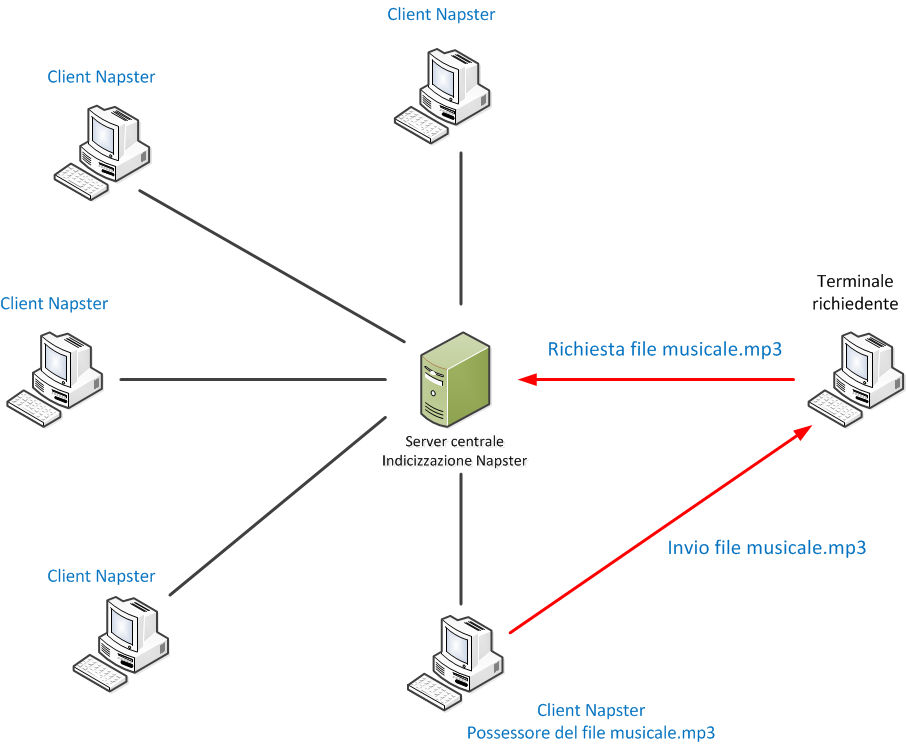
\includegraphics[width=15.3cm]{img/napster.png}
\end{center}
\caption{Architettura di Napster}
\label{Architettura Napster}
\end{figure}
Napster � stato il primo software di p2p ad avere una diffusione di un certo livello. Nacque nel 1999 da un progetto di Shawn Fanning.
Non era un sistema p2p puro, in quanto manteneva una lista di tutti gli utenti connessi e dei loro file su dei server centrali raggiungibili da tutti.
Quindi se un nodo voleva trovare un file mandava la richiesta al server centrale che rispondeva con la lista dei nodi che lo avevano e il richiedente poteva fare partire il download da tali nodi. Quando utente decideva di condividere un file mandava i dettagli al server centrale che li salvava.
Quindi le condivisioni vere e proprie avvenivano tra gli utenti, era come un programma di istant messaging avanzato.
I vantaggi di questo tipo di struttura risiedono nella velocit� di reperibilit� delle informazioni, in quanto l'elenco era disponibile a tutti direttamente. Altro punto a suo favore � la velocit� di condivisione, in quanto i nodi si scambiano i file creando una connessione diretta tra di loro, e il file � in chiaro e completo.Per� quelle che sono le sue caratteristiche positive in una prima analisi, si rivelano i suoi maggiori punti deboli se vista dalla prospettiva di utenti male intenzionati. Per esempio se il server centrale cade, tutta la rete smette di funzionare. Oppure se un ente vuole proibire la diffusione di certo materiale gli baster� confiscare il server per sapere chi ne era il detentore e con chi lo ha condiviso. Il connettersi direttamente con un altro utente porta inoltre tutta una serie di punti deboli, come la facile trasmissione di infezioni informatiche, il fatto che se il nodo � spento il file non � raggiungibile, la mancanza di certificati di autenticit� permette ad utenti di modificare contenuti e re immetterli in rete.
\subsection{Gnutella}
\begin{figure}
\begin{center}
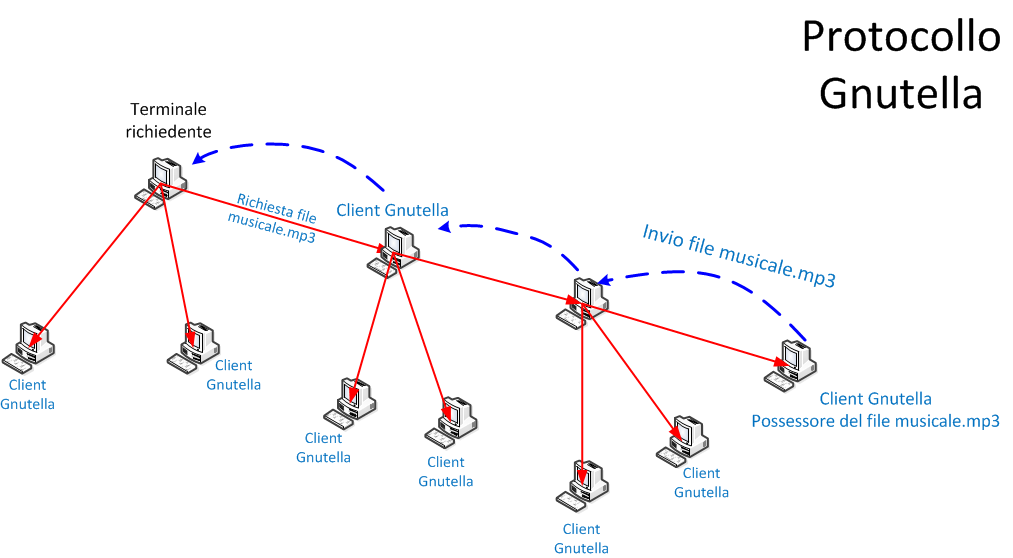
\includegraphics[width=15.3cm]{img/gnutella.png}
\end{center}
\caption{Architettura di Gnutella}
\label{Architettura Gnutella}
\end{figure}
Gnutella a differenza di Napster � un software peer to peer puro. Cio� non ha alcun server che centralizza alcun tipo di informazione.
I computer degli utenti sono gli unici nodi che compongono la rete. Quando un certo numero di utenti installa il software sulla propria macchina, automaticamente Gnutella riconosce i nodi vicini e e in questo modo la rete si amplia. Le ricerche avvengono secondo la tecnica del flodding, cio� un nodo per trovare un file manda una richiesta ai nodi vicini, se i nodi vicini non hanno il file richiesto inoltrano a loro volta a tutti nodi che conoscono la stessa domanda, tranne al nodo che gli ha mandato la richiesta originale. Per evitare il collasso della rete le richieste avevano un numero massimo di 'salti' tra nodi, al termine del quale venivano cancellate. Anche i trasferimenti di file vengono sostenuti dai nodi intermedi tra richiedente e possessore. 
Questo protocollo ha il vantaggio di essere potenzialmente inarrestabile, fortemente stabile e molto dinamico permettendo a nodi di entrare e uscire senza modificare le prestazioni della rete. Non teme quindi attacchi che ne arrestino il funzionamento. 
Per� la tecnica di ricerca molto rudimentale non garantisce di trovare un file, e i tempi per trovarlo comunque possono essere molto lunghi.
\subsection{Kademlia}
\begin{figure}
\begin{center}
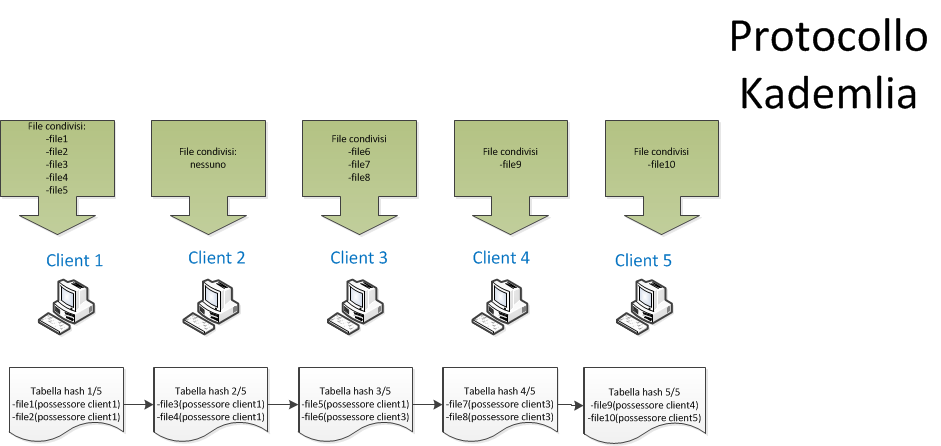
\includegraphics[width=15.3cm]{img/kademlia.png}
\end{center}
\caption{Indici dei file in Kademlia}
\label{Indici dei file in Kademlia}
\end{figure}
E' un protocollo di rete peer to peer decentralizzato ideato da Petar Maymounkov e David Mazi�res della New York University.
E' il primo protocollo che analizziamo che sfrutta la tecnologia delle DHT ovvero Distribuited Hash Tables.
Il metodo di mantenimento dell'indice dei file presenti sulla rete, DHT appunto, � il suo punto forte. Fino a quel momento il reperimento dei file era o totalmente centralizzato, mantenendo le liste in uno o pi� server, o totalmente distribuito, dovendo contattare moltissimi nodi per trovare i file.
Per capire come funzionino invece le DHT immaginate la lista di tutti i file presenti in una rete p2p, ora spezzettate questa lista in tante parti e distribuitele ai nodi che la compongono. E' chiaro che questi pezzi di lista sono replicati, in modo che se un nodo cade ve ne siano alcuni con la stessa informazione.
Ogni nodo oltre ad avere il suo pezzetto di lista sa anche in che direzione la lista si propaga, in questo modo se un nodo a lui vicino gli chiede dove si trova un file, e lui non lo sa, potr� indicargli in che direzione continuare a cercarlo. Una volta che il nodo richiedente trova nella lista il file che vuole, legge gli ip dei nodi che hanno il file e procede al recupero del file.
Il reperimento dei file in questo modo � molto pi� veloce di quanto non lo sarebbe in una rete completamente decentralizzata dove � necessario fare rimbalzare la richiesta verso moltissimi nodi.
Ed � anche pi� sicuro del metodo centralizzato, non solo dal punto di vista della privacy ma anche di stabilit� della rete stessa e di reperibilit� dei file.
Dato che non esiste nessun tipo di centralizzazione e i nodi sono responsabili dei file che caricano per�, se tutti i nodi che conoscono un file si spengono l'intera rete non riuscir� pi� a raggiungere quel file.
\subsection{Le darknet e Freenet}
\begin{figure}
\begin{center}
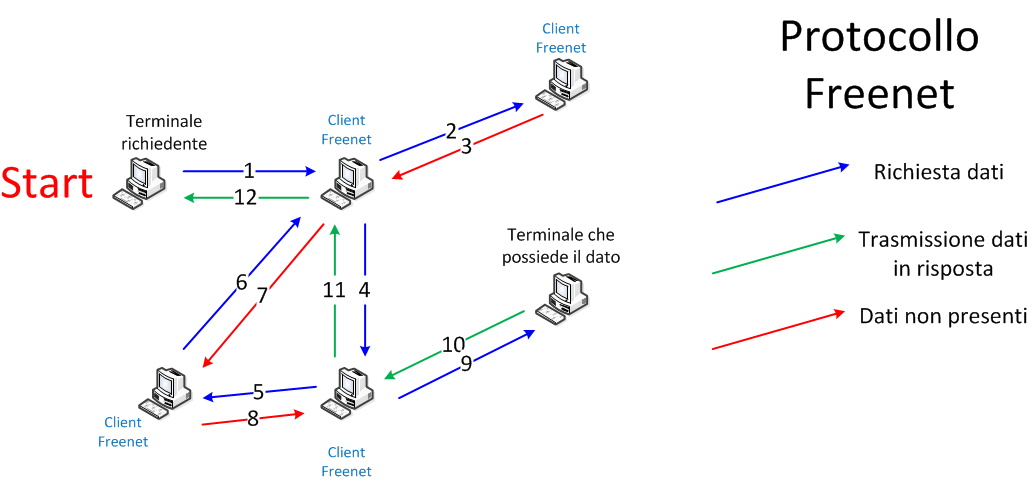
\includegraphics[width=15.3cm]{img/freenet.png}
\end{center}
\caption{Esempio protocollo Freenet}
\label{Protocollo Freenet}
\end{figure}

Le darknet sono reti per condividere file nate per tutelare la privacy e combattere la censura.
Infatti in alcuni paesi lo stato proibisce di condividere file che dicano cose che non sono da esso approvate, e per permettere la libera
diffusione di informazioni alcuni Informatici hanno pensato ad un modello di rete altamente dinamico e anonimo.
Il termine darknet � stato coniato prima della nascita di internet nel 1970, quando l'unica rete riconosciuta era ARPANET e identificava
una rete che fosse isolata da ARPANET per motivi di sicurezza. Questo per� non vuol dire che ne fosse separata, infatti i terminali che appartenevano a
quelle darknet potevano ricevere ed inviare dati attraverso ARPANET, ma non risultavano registrati da nessuna parte e non potevano essere rintracciati
in quanto non rispondevano ai segnali che chiedevano di identificarsi.
Con il tempo e l'avvento di internet si inizi� ad usare il termine darknet per indicare reti private, 
che per� passavano per internet, che alcuni utenti usavano per scambiarsi file, ma sempre e soltanto in piccoli gruppi di persone che si conoscevano.
Questo termine prima sconosciuto ai profani � stato dato in pasto ai media a seguito della pubblicazione di un documento \cite{thedarknet} da parte di quattro ricercatori della Microsoft.
Questo documento elencava tre punti essenziali che permettevano di identificare una rete come darknet: 
\begin{enumerate}
	\item ogni oggetto distribuito doveva essere condiviso sulle macchine di una parte degli utenti, in una forma che ne consentisse la copia
	\item tutti gli utenti possono ottenere una copia dei file se ne hanno interesse
	\item tutti gli utenti devono essere connessi tramite banda larga
\end{enumerate}
Questo documento fu condiviso su larga scala e interpretato dai tutori del diritto di autore come il principale impedimento alla diffusione 
di materiale protetto in forma elettronica.
Quindi si pu� spesso sentire parlare di programmi di condivisione come furono Napster, Gnutella, Kademlia e molti altri sotto la definizione di darknet da parte dei media, ma in realt� non � cos�. Questi sono programmi di p2p, peer to peer, differenti dalle darknet a causa della accessibilit� delle reti a chiunque installi semplicemente il software.
La tipologia di rete che si avvicinava di pi� al concetto di darknet erano le reti f2f, friend to friend.
Ovvero reti dove si era collegati solo a nodi fidati e conosciuti, tramite porte e protocolli non standard. 
Il concetto di darknet per� � stato ulteriormente rivoluzionato attorno al 2005 con la nascita di reti p2p ANONIME.
Reti nelle quali � possibile condividere file senza il rischio di essere rintracciati .
Proprio per questa caratteristica le reti darknet sono molto criticate, perch� oltre che per preservare la libert� di informazione pu� essere utilizzato per condividere materiale illegale e dannoso.

Il programma che abbiamo scelto di studiare nella categoria darknet � stato Freenet. Questa scelta � stata dettata dalla grande comunit� che gli sta alle spalle, dal fatto che sia disponibile il codice sorgente, e dalle caratteristiche che pi� si avvicinavano al nostro modello. Infatti Freenet � una rete decentralizzata, cio� dove non abbiamo server ma tutte le informazioni sono distribuite sui nodi. E' una rete realizzata puntando ad un alto livello di sicurezza ed anonimato. 
I file sono salvati sui nodi in modo crittografato e replicati su diversi nodi. Questo fa si che chi ha installato il programma non conosca cosa stia condividendo. Non esiste una struttura gerarchica tra i nodi, i collegamenti si basano sulla vicinanza, ogni nodo conosce solo quelli vicino a lui. Quindi quando vengono aggiunti nuovo nodi non si pu� prevedere a chi saranno collegati. Ogni file � contraddistinto da un id univoco, e il meccanismo per gestire l'indicizzazione dei file � simile alle DHT per� invece che basarsi su una lista dei file che un nodo possiede si basa sulla velocit� con la quale un nodo pu� avere un file. Dopo che un nodo ha trovato il file la richiesta passa di nodo in nodo, fino a raggiungere il nodo con il file. In seguito il nodo possessore del file lo invia, e il file viene trasmesso tra tutti i nodi intermedi. Quando vengono caricati nella rete i file non rimangono nel nodo che li ha condivisi, ma vengono replicati in modo da essere disponibili ad una certa velocit� per tutti i nodi della rete. Dato che il modo per indicizzare i file si basa sulla velocit� alla quale un file � disponibile questo vuol dire creare una ridondanza dei file su tutta la rete in modo da essere disponibili pi� velocemente per tutti! 
Oltre al funzionamento sulla topografia sopra descritta, cio� sfruttando tutti i pc con installato Freenet presenti sulla rete internet, il software offre una modalit� di funzionamento friend to friend. In questo setting noi andremo a specificare una lista di nodi manualmente, e i nodi inseriti saranno gli unici con cui andremo a condividere dei file.
E' una opportunit� in pi� tramite la quale si va a chiudere la rete dei propri amici. Pu� essere utile per esempio per alcuni gruppi di utenti che condividono file riservati e non vogliono renderli disponibili a tutta la rete Freenet.
Ogni caratteristica di questo programma � atta ad aumentarne l'anonimato e possiamo dire che funziona molto bene.
Tuttavia queste scelte sono state fatte essendo consapevoli che i file condivisi sarebbero stati documenti di piccole dimensioni. Questo rende lento e difficile la gestione di file di dimensioni maggiori, caratteristica che il nostro software deve avere.
\subsection{Cloud computing}
\begin{figure}
\begin{center}
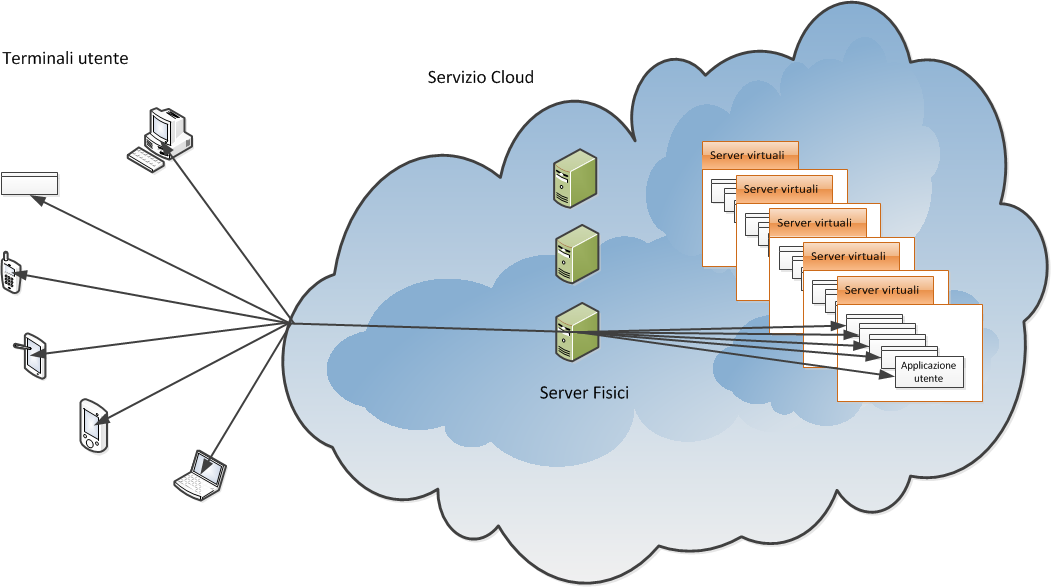
\includegraphics[width=15.3cm]{img/cloud.png}
\end{center}
\caption{Struttura Cloud Computing}
\label{Struttura Cloud Computing}
\end{figure}
Di cloud computing si sente parlare gi� dal 1960, quando lo scienziato informatico John McCarthy ipotizza un futuro nel quale la capacit� di calcolo sarebbe stato organizzato come un servizio di pubblica utilit�. Naturalmente i primi passi furono ben distanti, infatti le grandi aziende che con gli anni iniziavano ad usare data center avevano delle macchine che erano dedicate a sopperire solo alle richieste di un cliente. Gli studiosi si accorsero che per la maggior parte del tempo per� le macchine lavoravano al minimo, registrando picchi di calcolo solo in certi momenti della giornata. In questo modo per� vi era un enorme spreco di energia elettrica e di risorse inutilizzate. La prima multinazionale che notato questi sprechi si mise al lavoro per trovare una soluzione fu la americana Amazon. Infatti nel 2006 present� Amazon Web Service, che erano un insieme di servizi web. All'interno dei servizi proposti ve ne erano diversi di cloud computing, per esempio servizi che offrivano spazio online dinamico e veloce con costi in base al consumo, servizi che offrivano sistemi operativi virtuali utilizzabili online con costi basati sul tempo che si usavano e server per applicazioni web dove si pagava in base alle ore che il servizio era operante. E possiamo dire che � stata proprio questa la nascita del vero e proprio cloud computing, ovvero servizi web che ci offrono spazio di archiviazione, capacit� computazionale, sistema operativo, hardware e banda in base alle nostre esigenze in modo dinamico. Un po come la rete di distribuzione idrica o del servizio elettrico, dove si paga quello che si consuma. 

Negli ultimi tempi poi abbiamo visto una esplosione di questo tipo di servizi, infatti ormai quasi tutti i provider hanno a listino un servizio di cloud. Inoltre viste le potenzialit� molte aziende del calibro di Apple e Microsoft stanno utilizzando questa tecnologia per dare un servizio importante ai propri utenti come il centralizzare i dati personali tra i tanti terminali che oggi si hanno, notebook, desktop, smartphone, tablet. Possiamo dire che il cloud cambier� l'informatica da come la conosciamo adesso.

Il cloud computing � una risorsa molto preziosa visti i moderni strumenti che mette a disposizione, non solo perch� offre una grande potenza di calcolo o di spazio di archiviazione con un basso costo vista la dinamicit�, ma anche perch� i moderni strumenti usati dal cloud per virtualizzare ci permettono di avere un qualsiasi modello di hardware vogliamo subito e di fare le modifiche necessarie a piacimento.
Dato che la nostra rete darkcloud deve rendere i dati sempre disponibili, non era possibile scegliere una struttura di rete che mantenesse il dato sui client. Ci� avrebbe portato molti rischi che non potevamo accettare. Invece la tecnologia del cloud computing ci permette di avere una serie di macchine sempre online e con uno spazio di archiviazione e una banda passante di capacit� che vanno oltre il nostro massimo bisogno. 

\chapter{Progetto}
In questo capitolo si proceder� a illustrare le scelte progettuali, il funzionamento a livello logico funzionale del software e della rete che sta dietro darkcloud.
\section{Obbiettivi di dettaglio}
Come discusso nel capitolo precedente la sfida che ci � stata posta � stata di fornire ad un gruppo di professionisti uno strumento per poter
condividere file in modo sicuro. Questo richiede specifiche caratteristiche sia nelle scelte di progettazione della struttura di rete sia nelle scelte di soluzioni adottate nella programmazione del codice.

L'avvento del cloud computing ci ha dato uno strumento molto potente che volevamo sfruttare per questo progetto, lo studio delle tecnologie di condivisione di file, peer to peer, ci ha dato una visione di insieme di quello che nel corso del tempo � stata l'evoluzione di queste reti. Questo studio ci ha permesso di avere molti spunti per poi tracciare quello che sarebbe stato il disegno della nostra soluzione. 
La dinamicit� di alcune reti p2p pure, ad una prima analisi pareva una ottima soluzione, visto che ci avrebbe permesso di realizzare reti che si ampliassero in modo automatico e quindi non sarebbe stato necessario ogni volta che si aggiungeva un server o un client andare a riconfigurare tutti i nodi. Il problema della sicurezza per� in una soluzione del genere rendeva molto pi� complicato verificare che i nodi aggiunti fossero nodi fidati. In una architettura p2p pura inoltre il carico di lavoro � equamente distribuito su tutti nodi in maniera indistinta, questo per� nel nostro caso non sarebbe stato adatto, in quanto avendo a disposizione una grande potenza di calcolo e grande larghezza di banda da parte dei nodi cloud contenuti in grandi data-center avremmo inutilmente sobbarcato di lavoro i calcolatori degli utenti ultimi che devono invece solo caricare file e poi scaricarli.  Un altro aspetto che ci ha spinto a scartare l'approccio p2p puro � il carico di lavoro che avrebbe portato realizzare una soluzione altamente dinamica rispetto ad una soluzione statica. La programmazione di un software dinamico richiede molte pi� parti e una complessit� totale molto maggiore. Quindi bisogna chiedersi principalmente a chi � indirizzato il nostro tipo di software, quale sar� il suo bacino di utenza, se si intende farlo crescere in futuro e cosi via, cercando quindi di impiegare la giusta quantit� di risorse.
Non ha senso realizzare un software e una architettura che sopporti migliaia di utenti quando � specificamente richiesto che funzioni per poche decine di persone.

Oggi non � difficile utilizzare un server centrale per concentrare tutte le informazioni e i dati di una azienda, anzi � proprio quello che fanno la maggior parte delle grandi, medie e piccole realt�. Anche noi avremmo potuto adottare una soluzione di condivisione con server centralizzati, questo avrebbe reso pi� veloce la nostra rete e avrebbe permesso la condivisione di file di pi� grosse dimensioni, non ch� una spesa in termini di sviluppo e mantenimento molto inferiore.
Ma essendo la sicurezza il punto centrale del nostro progetto questa possibilit� � stata scartata a priori.
I rischi di tenere i dati tutti si alcuni server sono troppi. Per esempio affidando tutti i dati ad una compagnia di server si rischia che se la compagnia ha problemi tecnici o subisce attacchi i dati rimangano inaccessibili per un periodo di tempi o addirittura cadano persi. Ancora se la sicurezza della azienda venisse compromessa rischieremmo che male intenzionati si approprino dei nostri dati e che questi vengano diffusi.

La tecnologia delle DHT � molto interessante in quanto rappresenta una specie di compromesso tra il modello a server centralizzati e il modello totalmente distribuito.
Per� anche in questo caso abbiamo una difficolt� di programmazione notevole e un carico di lavoro dei nodi distribuito non in modo ottimale.

Freenet � il programma che pi� assomigliava all'idea che avevamo della nostra rete. La modalit� di lavoro friend to friend ci avrebbe permesso di usare solo i nodi che volevamo noi, la sicurezza era nettamente al di sopra di quella che ci necessitava, l'informazione in Freenet viene spezzettata in tante parti e inviata con ridondanza a nodi diversi, cifratura dei file e delle connessioni. A fronte di queste considerazioni avevamo preso in considerazione di utilizzare il codice di Freenet come base per sviluppare la nostra idea. Avevamo gi� determinato che la struttura della rete per sfruttare il cloud sarebbe dovuta essere di due livelli, server e client, inoltre i server non dovevano comunicare tra di loro e a seguito dello studio del codice di Freenet � stato chiaro che le modifiche necessarie sarebbero state pi� impegnative che sviluppare da zero un programma con le specifiche che avevamo ormai delineato. 

Il nostro software doveva essere prima di tutto realizzato con l'obbiettivo di funzionare ottimamente su servizi di cloud computing. Doveva basarsi su una topologia a due livelli, client e server, in modo da sfruttare le potenzialit� offerte dal cloud e alleggerire il carico dei nodi client. Non doveva basarsi su un solo server ma su diversi, in modo da poter attuare una splitting dell'informazione verso questi ultimi. 

Dato che quindi abbiamo avuto l'opportunit� di programmare da zero il software abbiamo deciso di renderlo pi� adattabile a future espansioni dal lato client. Invece che dare una classica veste grafica dalla quale gestire il programma, implementata nel client, abbiamo preferito creare un altra entit� di interfacciamento con l'utente. Infatti il nostri client non ha interfaccia grafica, ma viene comandato da messaggi xml. Per utilizzarlo noi abbiamo creato uno script in python da usare come terminale per inviare i comandi al client. Questo � solo un esempio di terminale, ma � utile perch� in futuro si potr� comandare il client tramite interfaccia web, piuttosto che con un applicazione per cellulari. 
\section{Struttura di rete}
\begin{figure}
\begin{center}
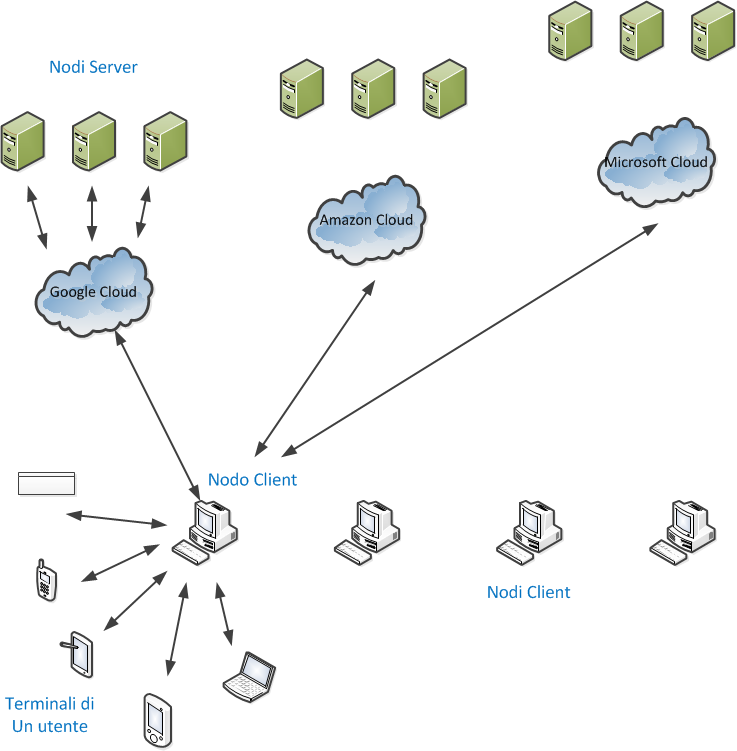
\includegraphics[width=15.3cm]{img/darkcloud.png}
\end{center}
\caption{Architettura di Darkcloud}
\label{Architettura Darkcloud}
\end{figure}
La rete Darknet � stata progettata con l'obbiettivo di proteggere i dati in essa condivisa.

La struttura di darkcloud si compone di tre tipi di nodi: i {\itshape server},i {\itshape client} e i {\itshape terminali}. 
I {\itshape  terminali} sono le interfaccie grafiche tramite le quali gli utenti interagiscono con il sistema.
I nodi {\itshape  client} sono quelli che eseguono le operazioni che gli utenti inviano tramite i terminali.
I nodi {\itshape server} sono i  delegati al mantenimento del'informazione, costituiti da istanze di cloud computing.
I terminali, i client e i server possono collegarsi tra di loro si tramite rete locale che tramite internet.
La topologia della nostra rete permette a diversi terminali dello stesso utente dicollegarsi ad un unico nodo.
{\itshape Fully connected} sul lato client, cio� tutti i nodi client possono comunicare tra di loro e con tutti i server.
Mentre invece il lato server pu� comunicare con tutti i client, ma i server non possono comunicare tra di loro.
Questo semplicemente perch� non � utile ai fini del loro compito. Mentre invece i client

Gli indirizzi dei vari nodi, sia client che server, sono specificati manualmente nella prima configurazione dei nodi. Quindi i nodi non si aggiungono dinamicamente. Dato le dimensioni contenute che la rete si propone di avere questo � stato pi� semplice e pi� sicuro di un approccio dinamico. Per identificare un nodo all'interno della rete si usa una chiave, che � un codice alfanumerico generato da una apposita funzione che ogni nodo conosce, funzione che ricevendo in ingresso l'ip e la porta del nodo restituisce in uscite la chiave di riconoscimento del nodo. In questo modo si crea un nuovo network virtuale sopra la rete internet.

Dopo aver avviato una certa quantit� di nodi server e alcuni nodi client, il nostro programma ci permette in modo trasparente di salvare un file nella rete.
Questo file viene elaborato da un protocollo, che si vedr� nel dettaglio nei paragrafi successivi.
Questo protocollo spezzetta i file e ne manda una parte ad ogni server.
Ora il nodo client ha riposto al sicuro il suo file, e pu� ricomporlo soltanto lui, quindi quello che pu� ora fare � condividerne la 
conoscenza con altri nodi o ad esigenza richiedere il file al programma.
Di primo acchito le perplessit� sulla sicurezza possono essere tante, ma si invita il lettore a leggere il paragrafo che parla 
della sicurezza del nodo.

I servizi di cloud computing che nella implementazione ultima andranno a mantenere i nostri file dovranno essere molteplici. Al momento se qualcuno ha bisogno di un certo numero di server su cui fare girare il proprio software pu� chiederlo direttamente ad un unico fornitore di servizi cloud. Per esempio per salvare i file in 100 parti diverse potrei chiedere ad un solo fornitore, uno tra Google Amazon Microsoft e altri, di caricare il mio software su 100 istanze che rappresentano sistemi operativi. A questo punto il mio file sarebbe salvato in parti sui server del fornitore scelto. Per� questo non sarebbe astuto per tutelare i dati del nostro professionista che li vuole mantenere al sicuro. In quanto essendo dati tutti a disposizione del fornitore nulla gli impedirebbe di ricomporre il file e di provare poi a decrittarlo. Se a questo punto il provider ottenesse i nostri dati potrebbe usarli per ricerche di mercato o profilazione degli utenti. Essendo spesso questi provider di servizi in paesi diversi dal nostro il tutelarsi in tali problemi di privacy diventa complicato. Oppure se un attaccante che trovasse una falla nei sistemi dello stesso fornitore potrebbe fare lo stesso. Ancora se affidiamo tutti i dati allo stesso fornitore in caso di malfunzionamento delle strutture i dati potrebbero essere irraggiungibili per un dato periodo di tempo. Per questi motivi si preferir� utilizzare diversi servizi di cloud computing per avere un certo grado di ridondanza dei dati e non lasciarli tutti nelle mani di un unico operatore.
\section{Architettura software}
\begin{figure}
\begin{center}
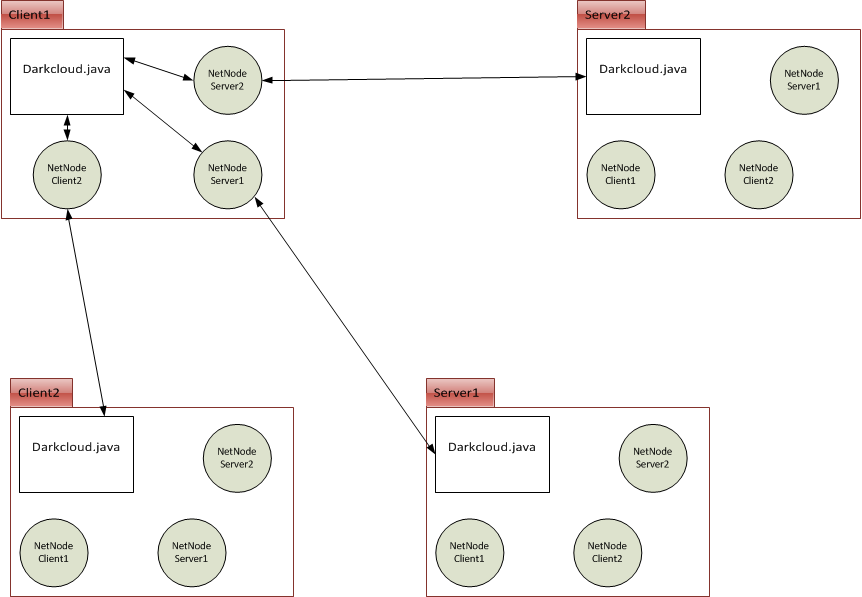
\includegraphics[width=15.3cm]{img/nodi.png}
\end{center}
\caption{Darkcloud e NetNode}
\label{Darkcloud e NetNode}
\end{figure}

Lo scopo di Darkcloud � quello di immagazzinare documenti in modo che nessuno che non abbia i permessi possa accedervi, permettendo anche di condividere il file tra pi� utenti.

Nel nostro software abbiamo 2 tipi di classi usati per identificare i diversi nodi della rete.
La classe Darkcloud.java e la classe Netnode.java. La classe Darkcloud.java � quella che ogni nodo istanza quando nasce. Invece le classi Netnode sono copie degli altri nodi, utilizzate per memorizzare in locale i dati degli altri nodi, come indirizzo, porta di ascolto e molto ancora.

Una nuova tecnologia che sta nascendo e di cui si sente molto parlare � il {\itshape cloud-computing}, grazie a questa tecnologia 
� possibile avere molte istanze di una applicazione senza dover per forza avere un server dedicato per ognuna di esse.
A patto di utilizzare le API di quel determinato fornitore di servizi cloud.
Infatti i metodi all'interno delle nostre classi sono stati sviluppati tramite la {\itshape reflection}, metodo di programmazione che ci permette di creare facilmente comandi incapsulati, in modo da poterli in un secondo momento adattare alle varie API dei diversi servizi di {\itshape cloud-computing} 
senza dover toccare il resto del codice.

Vista la continua evoluzione delle soluzioni hardware portatili come smartphone e tablet abbiamo pensato di fare evolvere anche il nostro software in modo da poterlo fare collaborare con queste tecnologie.
Infatti quando avviamo l'applicazione non � direttamente questa che andiamo ad usare per caricare i dati, ma sono dei terminali i quali poi contattano il client.
Per esempio al momento abbiamo sviluppato uno script in python che si chiama client.py tramite il quale, dopo aver avviato il nostro client, possiamo inviare ricevere e condividere file sulla rete. Adottando una soluzione del genere quando in un secondo momento, o a seconda di esigenze, si vorr� sviluppare una applicazione per tablet, o una applicazione web che ci permetta di usare la nostra rete da browser o ancora integrare l'uso della rete in altri software non sar� necessario andare a modificare il programma client ma semplicemente creare una interfaccia. Per poter rendere questo possibile il nostro utente dovr� avere un pc connesso ad internet che gestir� tutte le richieste che le sue diverse interfacce inoltreranno. Un po come un convogliatore di richieste ed invii. Questo rende molto pi� semplice lo sviluppo di nuove soluzioni per usare darkcloud.
\section{Protocollo di comunicazione tra nodi}
Le connessioni tra i vari nodi avvengono tramite connessioni criptate con il protocollo {\itshape SSL}. Il Secure Socket Layer, SSL, � un protocollo crittografico che permette una comunicazione sicura su reti TCP/IP, come nel nostro caso reti lan o internet. La cifratura avviene al di sopra del livello di trasporto. 
Questo protocollo consente alle applicazioni client/server di comunicare attraverso una rete in modo tale da prevenire il 'tampering' (manomissione) dei dati, la falsificazione e l'intercettazione.
L'autenticazione � bilaterale, cio� entrambi le parti si autenticano scambiandosi i certificati. Certificati che vengono generati alla creazione del nodo. In seguito questi certificati si scambiano tra i diversi nodi e tramite uno script apposito vengono aggiunti tra i certificati riconosciuti come 'trusted' per la nostra rete.

I messaggi che viaggiano tra i nodi criptati tramite SSL sono messaggi in formato XML. Questo formato � stato scelto perch� permette in maniera molto semplice di aggiungere al messaggio campi e attributi. 

I messaggi XML scambiati si dividono principalmente in due tipi: i messaggi Request e i messaggi Response. Quando un nodo vuole comunicare con un altro crea un istanza di un oggetto request, successivamente specifica di che tipo di richiesta si tratta, aggiunge i campi con le informazioni necessarie affinch� il nodo ricevente possa soddisfare la richiesta, e tramite il metodo send invia il messaggio all'altro nodo. Il metodo send si preoccupa di creare la connessione con il secondo nodo e di raccoglierne la risposta cio� un messaggio contenente un oggetto response che contiene la risposta del secondo nodo. Infatti una volta che il nodo ricevente ha la richiesta si preoccupa di vedere di che tipo si tratta, e in base a quello esegue il codice corrispondente a quel tipo di richiesta. Elabora i dati contenuti nella richiesta, crea una istanza di response, ci mette i risultati e li invia al richiedente.

I tipi di messaggi che i nodi si possono scambiare sono:
\begin{itemize}
	\item PING
	\item PUT
	\item GET
	\item SHARE
	\item RECEIVE
\end{itemize}

Il primo comando che andiamo ad analizzare � il PING.
Questo tipo di request viene usato dai nodi per verificare se gli altri sono online e quanto sono distanti calcolando i tempi di latenza.
Infatti � un comando che pu� essere usato anche dal nostro script client.py per verificare se i nodi client, tramite i quali possiamo mandare i file sulla rete, sono vivi. Ancora i nodi client effettuano un ping regolarmente verso i server in modo che quando devono caricare file sulla rete sappiano gi� quanti server sono disponibili e quindi in quante parti possono suddividere il file. Oltre a effettuare il ping regolare dei server si effettua anche quello degli altri client, in modo da effettuare le condivisioni dei file con loro in modo veloce. 
\section{Salvataggio e recupero dei file}
\begin{figure}
\begin{center}
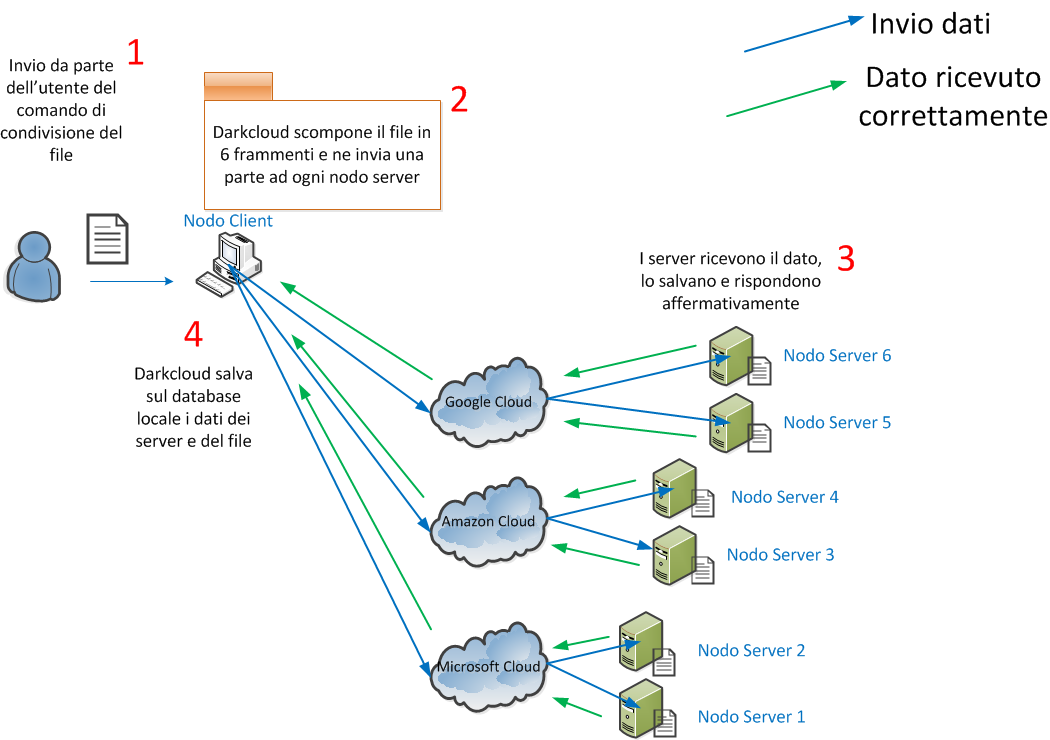
\includegraphics[width=15.3cm]{img/put.png}
\end{center}
\caption{Invio di un file su Darkcloud}
\label{Invio di un file su Darkcloud}
\end{figure}
Quando uno dei nostri client decide di caricare un file sulla nostra rete darkcloud, utilizza il comando PUT. Come abbiamo accennato prima parlando dell'architettura del software, noi abbiamo un interfaccia o molteplici, tramite le quali possiamo comandare il nostro client. Quando inviamo da un interfaccia un comando per salvare sulla rete il file, dal nostro script client.py per esempio,specifichiamo il nome del file locale, il nome con cui vogliamo che il file venga salvato e il client che dobbiamo usare. L'interfaccia specificher� quindi al client che abbiamo indicato il contenuto del file e un comando di put tramite un messaggio XML, il nostro client controller� prima l'integrit� del file poi lo cripter�, con specifiche che vedremo in dettaglio nel prossimo capitolo. Dopo di che in base a quanti server il client avr� a disposizione frammenter� il file in tante parti quanti sono i server. Proceder� poi a preparare tanti oggetti request quanto sono i frammenti, nei quali specificher� che si tratta di messaggi put, quale � il contenuto del file, il checksum per controlli di integrit� e infine invier� la richiesta ai server con il metodo send. Accertandosi che i server rispondano in maniera affermativa di aver ricevuto il frammento e di averlo correttamente salvato.Per poter ricomporre il file il client salver� su un database interno i dettagli dei file e di ogni frammento, compreso il checksum di ognuno e il nodo server sul quale � stato salvato.
\begin{figure}
\begin{center}
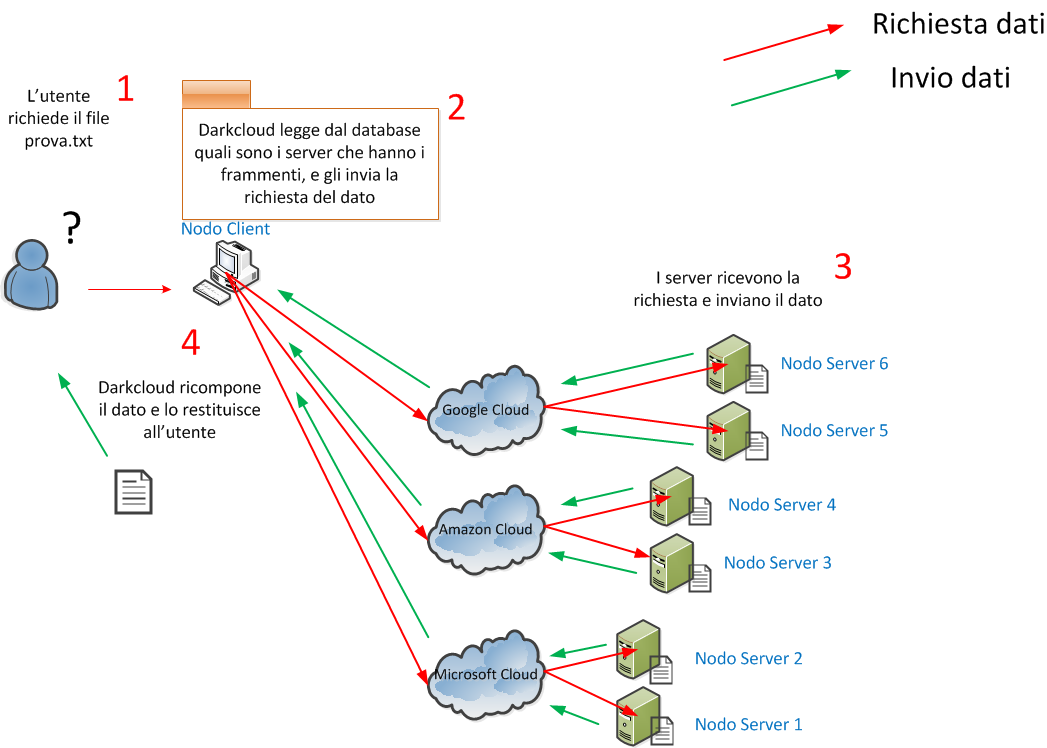
\includegraphics[width=15.3cm]{img/get.png}
\end{center}
\caption{Recupero di un file da Darkcloud}
\label{Recupero di un file da Darkcloud}
\end{figure}

L'operazione di recupero viene effettuata dalle interfacce. Nel caso del nostro client.py dobbiamo specificare il client che vogliamo usare, e il nome con il quale il file � salvato in remoto. Quindi l'interfaccia client.py invier� al client una richiesta di tipo GET specificando il nome del file.
Il client a sua volta ricevuta la request recupera il campo con il nome e va a cercare nel sua database i dettagli di come e dove � stato salvato il file. Quindi su quali server, in quale ordine e quali sono i checksum delle singole parti. Una volta inviate le request ai server specificando i nomi dei frammenti, recupera le response mandate dai server. Ora pu� controllare l'integrit� dei file calcolando il checksum dei frammenti ricevuti e confrontandolo con il checksum che aveva salvato. Se i dati sono corretti ricompone il file e lo decripta, inviandolo per concludere all'interfaccia che glielo aveva richiesto.

\section{Condivisione dei file}
\begin{figure}
\begin{center}
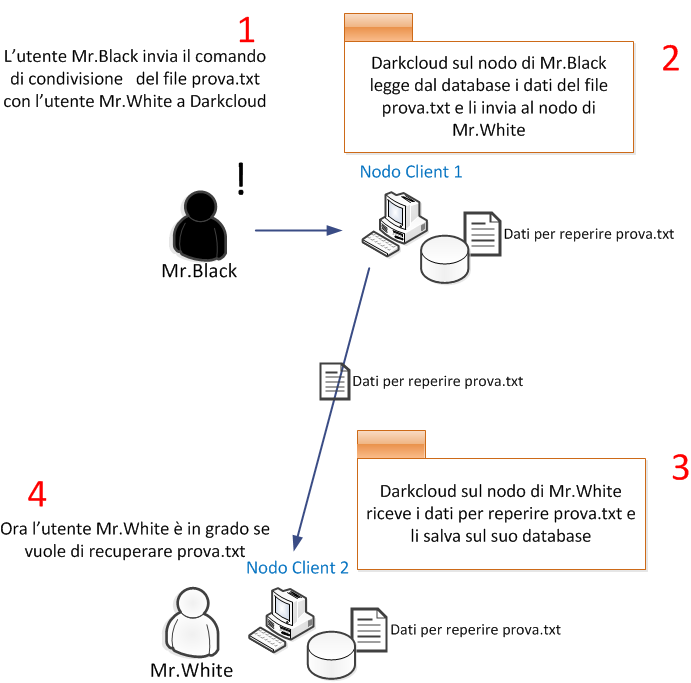
\includegraphics[width=15.3cm]{img/share.png}
\end{center}
\caption{Condivisione di un file con un altro utente}
\label{Condivisione di un file con un altro utente}
\end{figure}
Fino ad ora abbiamo visto a grandi linee il funzionamento del salvataggio e del recupero del file, ma dato che questa rete deve permettere a persone di condividere tra di loro file � stato anche implementato un comando SHARE. Questo comando non va a toccare i server, in quanto non avrebbe avuto senso replicare i file sulla rete per ogni utente, infatti quello che abbiamo permesso con il comando share � stato la condivisione della conoscenza di un comando con un altro nodo.
Se un ipotetico utente1 volesse condividere un file con l'utente2 sar� sufficiente usare il comando share.
Dato che la conoscenza e i dati sono salvati sul client e non sulle interfacce, sar� l'utente1 che chieder� tramite la sua interfaccia al suo client di inviare al client di utente2 i dati riguardanti un determinato file. In modo che in un secondo momento se l'utente2 vuole recuperare il file possa semplicemente chiederlo al suo client tramite la sua interfaccia. La procedura parte con l'utente1 che invia tramite la sua interfaccia un richiesta al suo client specificando il nome del file remoto, e i parametri del client di utente2, nel nostro caso specifico di client.py per esempio si tratta dell'indirizzo ip e della porta di ascolto. Il client di utente1 andr� a recuperare dal suo database tutti i dati necessari a recuperare il file. Ora creer� un oggetto request di un tipo RECEIVE e gli allegher� tali dati. Il comando receive serve per salvare nel database locale  i dati di un file, e dei suoi frammenti, che non � stato caricato nella rete dal nodo che esegue il comando. Quindi a seguito della ricezione dei dati e dell'esecuzione del comando receive il client dell'utente2 sar� in grado come l'utente1 di recuperare il file.
\section{Sicurezza del nodo}
E' vero che il mantenere l'indice di tutti i propri file in locale potrebbe essere un punto debole sul piano della sicurezza, ma proprio per questo abbiamo con una serie di accorgimenti reso molto difficile per un attaccante, anche qual'ora avesse compromesso il nodo, reperire le informazioni.
Questo � possibile grazie all'utilizzo combinato , di crittografica simmetrica, crittografia asimmetrica, invio dei dati ai server in modo casuale, utilizzo di comunicazioni criptate secondo il protocollo SSL, controllo in ogni operazione dell'integrit� dei file tramite checksum e aggiunta di nodi in modo statico. 

Infatti quando un file � stato spezzettato, ogni parte viene cifrata e poi inviata ai server. 
Se l'invio ai server avvenisse in modo sequenziale e ordinato, un utente che stesse sniffando la nostra connessione riceverebbe i frammenti in ordine facilitandogli notevolmente il lavoro di ricostruzione. Ancora se mettessimo i file in modo ordinato in base ai server chi avesse accesso a questi server potrebbe sapere in che ordine andrebbero riordinati.
Per evitare ci�, dopo aver spezzettato il file e salvato sul database la sequenza esatta il programma mescola i frammenti tra di loro, solo dopo questo li invia ai server.

Per verificare che i dati che vengono scambiati tra i nodi non vengano contraffatti o subiscano modifiche a causa di errori di connessione si � fatto un forte uso dei controlli del checksum. Il checksum � una sequenza di bit che viene calcolata partendo da un file. Il checksum di un file � univoco, quindi se il file viene modificato il checksum non corrisponde pi�. Prima di inviare un frammento di file ad un server, ad esempio, un client ne calcola il checksum e lo salva sul database. Oltre a ci� salva anche il checksum dell'intero file. Quando in un secondo momento andr� a ricomporre il file, dopo aver recuperato i frammenti andr� a calcolare i checksum di tali frammenti e li confronter� con i checksum salvati. Stesso procedimento dopo aver ricomposto il file, ne calcoler� il checksum e lo confronter� con quello salvato. Questo ci aiuta anche ad evitare errori nelle procedure di ricomposizione dei file.

\subsection{Crittografia}
La crittografia asimmetrica, conosciuta anche come crittografia a coppia di chiavi, � un tipo di crittografia usata per condividere file tra due o pi� utenti. Questo tipo di crittografia permette agli utenti di scambiarsi informazioni in modo che un terzo utente non autorizzato non possa leggere il messaggio. Ogni utente in questo sistema possiede due chiavi di cifratura, una pubblica e una privata. La chiave pubblica viene data a chiunque voglia comunicare con lui, mentre quella privata rimane di esclusiva conoscenza del proprietario. Un messaggio cifrato con la chiave pubblica dell'utente1 pu� essere decifrato solo tramite la chiave privata dell'utente1. In questo modo se l'utente2 vuole mandare un messaggio cifrato all'utente1, lo cifrer� con la sua chiave pubblica, e solo l'utente1 potr� leggerlo. 
Nel nostro caso abbiamo usato questo metodo per cifrate le parti di file che vengono scambiate tra i nodi. Ogni nodo ha la sua chiave privata e quella pubblica, e inoltre tutti i nodi conoscono le chiavi pubbliche degli altri. In questo modo quando si condividono parti di file tra nodi client e server un male intenzionato che intercettasse i nostri pacchetti non riuscirebbe a carpirne l'informazione. 
I file invece prima di essere spezzettati vengono criptati tramite una chiave simmetrica creata dal nodo stesso. La crittografia simmetrica permette di criptare un file con una chiave, e per decriptare quel file quella chiave � l'unica utilizzabile. In modo che anche se un male intenzionato riuscisse a ricomporre il file infrangendo la crittografia asimmetrica, dovrebbe avere un ulteriore chiave per decifrare il file intero.
Dato che ogni nodo mantiene l'indice dei file in locale, prima di salvare le chiavi di cifratura simmetrica sul database, queste chiavi vengono ulteriormente cifrate tramite la chiave pubblica del nodo locale. In questo modo se qualcuno riuscisse a rubarci il database, senza la nostra chiave privata non riuscirebbe a conoscere le chiavi dei nostri file.

\chapter{Soluzioni basso livello}

In questo capitolo procederemo ad una disamina delle scelte tecniche fatte nel progetto darkcloud, e illustreremo il funzionamento dettagliato delle procedure.

\section{Linguaggi di programmazione e ambiente di sviluppo}
\begin{figure}
\begin{center}

\includegraphics[width=15.3cm]{img/logo.png}
\end{center}
\end{figure}
Il linguaggio con il quale � stato scritto darkcloud � Java\cite{java}. La scelta � stata orientata verso questo linguaggio dopo considerazioni fatte sulla complessit� del codice di cui si necessitava. Infatti dato che abbiamo optato per un software dove le chiavi di decriptazione, le informazioni su tutti i file, i dati degli altri nodi e molti altri dati sensibili sono salvati in locale si rendeva necessario adottare nel software forti mezzi per mantenere in sicurezza queste informazioni. In java gli strumenti per criptare sono di facile utilizzo. Inoltre anche le connessioni e la formattazione dei messaggi scambiati tra nodi risultava molto semplificata grazie alle classi gi� disponibili. Dato che si doveva costruire da zero una piattaforma per gestire una rete e questa avrebbe avuto bisogno di un codice molto articolato e con elementi con metodi simili ma caratterizzazioni diverse, ha reso java una scelta preferibile. Il software che realizzavamo doveva poi essere in grado di essere eseguito su piattaforme di diverso tipo, in quanto non solo i professionisti che lo usano potrebbero eseguirlo su sistemi operativi diversi, ma visto che ne saranno usate istanze su cloud computing e facile che lo si eseguir� in queste ultime su sistemi linux.
Oltre al linguaggio java nel software utilizziamo l'sql per salvare i dati. In particolare abbiamo utilizzato il client sqlite3, dato che il nostro software deve salvare informazioni su molti altri nodi, su ogni file , e per ogni file sui frammenti � indispensabile un linguaggio di gestione database multi piattaforma e stabile come l'sql.
Una scelta ormai assodata del gruppo di lavoro del professor Colajanni � l'utilizzo del sistema operativo Debian per la fase di sviluppo del software. Tale sistema operativo infatti garantisce nelle release stable la sicurezza di lavorare su un sistema molto stabile e nella comunit� degli sviluppatori molto sfruttato. Essendo usato molto dai programmatori gli strumenti di compilazione, debug, e gli ambienti di sviluppo per programmare sono stati testati a lungo e quindi arrivati ad un buon livello di stabilit�. Essendo sicuri che non dar� spiacevoli sorprese in corso di programmazione. 
L'ambiente di sviluppo java utilizzato � stato Eclipse. Gli strumenti che offre per il lavoro di programmazione sincronizzato lo rendono perfetto per il nostro caso, nel quale io e il correlatore della tesi, l'ingegner Fabio Manganiello, abbiamo lavorato simultaneamente sul codice.
Per sincronizzare il codice abbiamo usato Google Code. Si tratta di un servizio di casa Google gratuito che permette di creare progetti software e consente a diverse persone di lavorarci. Abbiamo infatti installato il plugin Subversion per Eclipse, questo ci ha permesso di impostare il repository per il progetto. In questo modo chi lavora ad una classe pu� bloccarla direttamente da Eclipse e quando ha finito sbloccarla e caricare i risultati. 
Quindi i requisiti di sistema sono una installazione di Java Runtime Environment versione 1.6.x o maggiore e il client di sqlite3.
\section{Analisi di un nodo}
Per funzionare un nodo, che sia client o server, ha bisogno di alcuni file. 
Il file eseguibile darkcloud.jar, che � lo stesso sia per i client che per i server. Questo eseguibile deve essere avviato sia sui client che sui server. Una volta avviati almeno un client e un server sar� possibile iniziare ad usare il sistema tramite un terminale, potendo salvare file e recuperarli.
Il database darkcloud.db, che contiene tutte le informazioni del nodo. Nel database vengono salvati i dati di tutti i file, i dati dei frammenti dei file e le caratteristiche degli altri nodi presenti in darkcloud.
Il file di configurazione darklcoud.conf, che contiene tutti i setting del nodo. Vi troviamo specificati l'indirizzo ip e la porta di ascolto del nodo locale, il tipo di nodo locale, l'indirizzo ip e le porte degli altri nodi presenti sulla rete con specificato se si tratta di client o server.
Il file darkcloud.keystore, che contiene le chiavi pubbliche degli altri nodi e i certificati ssl. Dato che nella rete utilizziamo connessioni protette SSL ogni nodo deve conoscere la chiave pubblica di ogni altro nodo, oltre a ci� le chiavi pubbliche degli altri nodi sono usate per cifrare i file che gli si mandano.
Infine i file private.key e public.key che contengono le chiavi RSA pubblica e privata del nostro nodo usate per criptare e decriptare le informazioni da e per il nodo.
Se si vuole spostare un nodo su un altro computer sar� sufficiente spostare i file sopra menzionati. Dato che la mappatura dei nodi � contenuta nel file darkcloud.conf dovremmo anche modificare i valori se cambier� l'ip del computer in uso, sia nelle impostazioni locali che nelle liste ip degli altri nodi che devono comunicare con noi.
\section{Gestione dei nodi}
Per gestire i nodi sono stati creati una serie di script che permettono di eseguire le funzioni fondamentali per il funzionamento della rete. Sono script da usare solo per modifiche da parte di amministratori della rete, gli utilizzatori finali non si troveranno mai a doverli usare dovranno solo interagire con i terminali. Questi script si possono trovare nella sotto directory 'net' e sono:
\begin{itemize}
	\item createNode.sh 
	\item removeNode.sh
	\item startNet.sh
	\item stopNet.sh
	\item startNode.sh
	\item stopNode.sh
\end{itemize}
Lo script createNode.sh permette di creare dei nodi, i parametri richiesti quando viene avviato sono: nome del nodo, tipo di nodo che pu� essere client o server, porta di ascolto, keystore password, nome e cognome, nome dell'unit� aziendale, nome dell'azienda, localit�, provincia, codice a due lettere del paese in cui si trova l'unit�. Al temine della configurazione lo script controlla se sono gi� stati creati altri nodi. Successivamente ci viene chiesto se vogliamo che i certificati degli altri nodi che sono stati trovati siano marcare come fidati, questo � necessario se vogliamo essere in grado di comunicare con essi. Al termine di questa operazione della sotto directory 'net' avremo una cartella che si chiama come il nostro nodo contenente i file necessari al suo funzionamento.
Le impostazioni precedentemente inserite vengono salvate nel file di configurazione del nodo chiamato darkcloud.conf . Se in seguito alla creazione si vuole apportare modifiche al nodo baster� andare nella directory 'net', nella sotto directory che si chiama come il nodo e modificare tale file. 
In particolare di default tutti i nodi conosciuti e certificati della rete hanno 127.0.0.1 come indirizzo ip. Se si vuole spostare questi nodi su altre macchine collegate ad internet, basta poi modificare i file darkcloud.conf di tutti i nodi della rete.
Infatti la conoscenza che un nodo ha degli altri � specificata in tale file, quindi se la geografia della rete viene cambiata deve essere aggiornata in ogni nodo della rete. 
Lo script removeNode.sh ci permette di disinstallare il nodo dalla macchina locale, e si occupa anche di rimuovere da eventuali altri nodi presenti nella cartella le specifiche del nodo rimosso.
Con lo script startNet.sh possiamo avviare tutti i nodi presenti nella directory 'net'. Se invece si vogliono avviare dei nodi singolarmente si utilizzer� lo script startNode.sh. 
Quando un nodo viene avviato in una cartella nascosta che si chiama .run vengono creati dei file nel formato 'nome nodo'.pid nei quali vengono salvati i pid dei nodi avviati. Questo serve per evitare di aprire pi� istanze dello stesso nodo, azione che porterebbe a problemi sul database e alla gestione delle risorse. Al loro avvio gli script di avvio della rete o dei nodi controllano che nella cartella .run non ci siano gi� i pid dei nodi che si tenta di avviare. Inoltre gli script di avvio controllano che all'interno della cartella del nodo siano presenti l'eseguibile e il file di configurazione per evitare errori.
Analogo discorso per lo script stopNet.sh tramite il quale possiamo spegnere tutti i nodi presenti nella directory 'net'. Mentre se si vuole spegnere un singolo nodo si utilizzer� lo script stopNode.sh. Oltre a inviare il segnale di kill del processo gli script di arresto cancellano dalla cartella .run i pid dei processi.
\section{Gli oggetti Darkcloud e NetNode}
Quando noi avviamo l'eseguibile di darkcloud, il main crea una istanza della classe Darkcloud e una della classe NetService. Darkcloud � la classe principale di ogni nodo, che contiene le variabili con le chiavi per la criptazione, le liste con i dati degli altri nodi, il collegamento con il database e altro ancora. NetService invece � la classe che prende i dati di ip e porta di ascolto del nostro nodo e crea il socket ssl che viene usato in ascolto. A seconda che un nodo sia client o server poi viene creata una istanza di ServerService o ClientService, che rimangono in ascolto di connessioni in entrata e in caso arrivino richieste istanziano a loro volta le classi Client o Server che si occupano di leggere il messaggio in arrivo e decifrare di che tipo di richiesta si tratta, invocando poi il giusto metodo di risposta delle classi ServerResponseMethod o ClientResponseMethod. Queste ultime due classi contengono il codice che un nodo esegue in risposta ad una richiesta. I dettagli del codice eseguito nei diversi comandi verr� analizzato nel paragrafo dedicato ai comandi. Le diverse richieste sono elencate all'interno della classe Request.java, che modella le richieste che i nodi possono scambiarsi. Attraverso il tipo di Java definito Enum, Enumerazione, possiamo nella classi Request.java definire i diversi tipi di richieste semplicemente specificandone il nome, in modo che nelle classi ServerResponseMethods.java e ClientResponseMethods.java andiamo a indicare il codice da eseguire a seconda della richiesta ricevuta.
Se si vuole aggiungere un comando basta aggiungerlo alla lista lista in Request.java e scriverne il codice nella classe di risposta del client o del server.

La classe Darkcloud contiene due paricolari hashmap, chiamati clientNodes e serverNodes. Una hashmap � una collezione di oggetti, che memorizza coppie chiave-valore, dove la chiave serve come indice. clientNodes e serverNodes infatti sono composti da oggetti di tipo NetNode e chiavi di tipo stringa. Gli oggetti NetNode sono istanze della classe omonima e vengono create come immagini degli altri nodi della rete, utilizzate quindi dalla classe Darkcloud come interfacce per comunicare con gli altri nodi.
La classe clientService oltre ad aspettare le connessioni in arrivo crea all'avvio un istanza della classe NetPoll. Questa classe viene fatta partire all'inizio del programma e rimane attiva sempre fino a quando non viene terminato il programma, il suo compito � quello di controllare periodicamente quali nodi sono vivi e quali no. Fa questo inviandogli dei messaggi di tipo ping, e in base alla risposta segna gli oggetti NetNode come online o offline all'interno della struttura clientNodes e serverNodes. 
La classe NetNode possiede un metodo che si chiama send. Questo metodo viene invocato dal nostro programma quando ha bisogno di inviare informazioni a un altro nodo. 
Il metodo send accetta in ingresso un oggetto di tipo Request e fornisce in uscita un oggetto di tipo Response. Dato che il nostro nodo costituito dalla classe Darkcloud, ha per ogni altro nodo un oggetto NetNode, all'interno del quale sono contenute le informazioni dell'altro nodo, se vogliamo inviare un messaggio all'altro nodo sar� sufficiente usare il comando NetNode.send. Ora il NetNode si attiver� e il suo metodo send legger� i suoi dati, creer� una connessione con il nodo remoto che lui rappresenta, gli invier� l'oggetto request che Darkcloud cio� il nodo locale gli vuole mandare, aspetter� la risposta rappresentata da un oggetto response e la restituir� a chi lo ha invocato cio� Darkcloud.
\section{Connessioni}
In questo paragrafo parleremo delle connessioni che instauriamo tra due nodi, tramite i quali scambiamo informazioni. Nel nostro caso specifico abbiamo deciso di utilizzare le connessioni SSL. Le connessioni SSL sono connessioni criptate tramite una chiave pubblica. Quando noi creiamo i nostri nodi, lo script di creazione crea per ogni nodo una coppia di chiavi e un KeyStore. Il KeyStore � un file che contiene tutte le password pubbliche degli altri nodi che appartengono alla rete. Questo KeyStore per sicurezza � a sua volta protetto da una password. Quando il nostro programma viene avviato sappiamo che la prima classe, quella principale, che viene istanziata � Darkcloud. All'interno di questa classe nei comandi di inizializzazione vengono impostate due variabili di sistema di java, javax.net.ssl.keyStore e javax.net.ssl.trustStore. In queste due variabili andiamo a porre la posizione del KeyStore, in modo che quando nel corso del programma andremo a creare un socket SSL java sappia dove pu� reperire la chiave del nodo che vogliamo contattare e in questo modo creare la connessione protetta.

L'avere una connessione per� non � sufficiente a trasferire gli oggetti che noi abbiamo ideato per passare i dati tra una classe e l'altra. Infatti il protocollo SSL trasporta stringhe mentre noi abbiamo bisogno di passare tra nodi diversi molti tipi di informazioni diverse, come numeri interi, byte di dati, date e altro. Per questo ci avvaliamo di una particolare formattazione delle stringhe che poi verranno scritte nei socket. In modo che quando il dato da noi inviato viene ricevuto da un altro nodo lui sappia come interpretarlo e quindi possa estrarne i contenuti informativi. Per formattare i nostri messaggi utilizziamo l'XML. XML � un linguaggio di markup, ovvero un linguaggio che definisce un meccanismo sintattico che ci permette di definire e riconoscere il significato degli elementi contenuti in un testo. 

Quando due classi vogliono scambiarsi informazioni lo fanno essenzialmente tramite l'uso di due oggetto, la request e la response. Request e response sono estensioni della classe message. La differenza tra di loro � che una request deve richiamare un comando, mentre la response deve comunicare se l'operazione � andata bene o male. Dato che i comandi dei nostri nodi sono cinque anche le tipologie di request sono cinque, mentre i tipi di response sono due, risposta positiva o errore.
Il codice degli oggetti request e response ha dei metodi che ci permettono di inserire al loro interno tutte le informazioni che vogliamo, e anche di organizzarle. Tramite il metodo appendField noi possiamo creare un nuovo campo, in questo campo possiamo inserire direttamente dei dati, oppure creare al suo interno degli attributi, tramite il metodo setContent. Quando abbiamo finito di inserire i campi e gli attributi le informazioni all'interno dei nostri oggetti sono pronte per essere spedite. Per fare questo utilizzeremo il metodo delle request e delle response che si chiama toString. Questo metodo prende tutti i dati che abbiamo riposto nel nostro oggetto, che abbiamo organizzato in campi e attributi, e lo converte in messaggi XML dovutamente formattati, sotto questa forma i nostri dati possono viaggiare sul socket SSL.
Una volta ricevuto questo messaggio XML potr� facilmente essere trasformato nell'oggetto originario, request o response che sia. Questo avviene creando un nuovo oggetto request o response e fornendogli il messaggio tramite il metodo fromString. Dato che l'oggetto sa come sono formattai i dati in XML pu� agilmente convertirli nei campi e negli attributi originali. 
In questi messaggi XML prima di essere spediti viene inserita la lunghezza del messaggio e la firma del mittente. Questo per facilitare la decodifica al metodo ricevente. Pi� precisamente � un messaggi formattato in 3 righe, nella prima riga c� la lunghezza del messaggio, nella seconda riga il contenuto informativo e nella terza riga la firma del mittente. 

I metodi che gestiscono la scrittura di questo messaggi sui socket sono il send di NetNode e run di CLient.
Quando un nodo vuole mandare un messaggio ad un altro nodo utilizza il metodo send all'interno dell'istanza NetNode che rappresento il nodo ricevente. Mentre il meccanismo di ricezione � basato sulla classe ClientService o ServerService. Queste classi sono continuamente in ascolto e se rilevano un messaggio SSL istanziano Client e gli passano il socket. Sia nel caso del send che del Client per prima cosa si creano due buffer uno per la lettura e uno per la scrittura. Nel send poi si allega alla request il campo nodeid, che comprende il proprio ip e la propria porta di ascolto, in modo che il ricevente abbia sempre i dati per identificare il mittente. 
Si procede poi a scrivere sul buffer uscente il messaggio XML tramite il comando request.toString() di cui abbiamo parlato prima che traduce il contenuto della request in codice XML. 
A questo punto il clientService o il serverService rilevano il messaggio, istanziano Client o Server e gli passano il riferimento al socket. Il Client per prima cosa legge la prima riga passata nel messaggio, che contiene la lunghezza, questo valore gli serve per decifrare il resto del messaggio. Ora legge dal buffer una riga lunga quanto era specificato nella prima riga. Forniamo in ingresso al metodo fromString, di un nuovo oggetto request, la stringa appena letta, i cui valori vengono cosi inseriti nella request stessa. Il Client ora salva in un array tutti i metodi che conosce il client, e poi li confronta con quello della request. Se trova una corrispondenza invoca tale metodo e gli passa l'oggetto request. Come risultato del codice del comando gli viene restituito un oggetto response, che procede a spedire sullo stesso socket dal quale ha letto tramite per� un buffer di scrittura. Chiaramente per scriverlo usa il metodo toString dell'oggetto response ricevuto che traduce il contenuto in una stringa. Infine Client chiude i due buffer e il socket. 
Il send riceve il messaggio tramite il socket, chiude il socket, traduce il response con fromString, chiude i buffer e il socket. Procede al controllo dell'esistenza del campo nodeid per verificare l'identit� di chi gli ha risposto. Dopo di che controlla anche il campo che contiene la chiave pubblica, e controlla se corrisponde con quella che il nodo ha salvato in corrispondenza di quel nodeid. Se cos� non � sostituisce la chiave con quella ricevuta. Per concludere restituisce l'oggetto response alla classe che lo aveva invocato. 
\section{Database}
\begin{figure}
\begin{center}
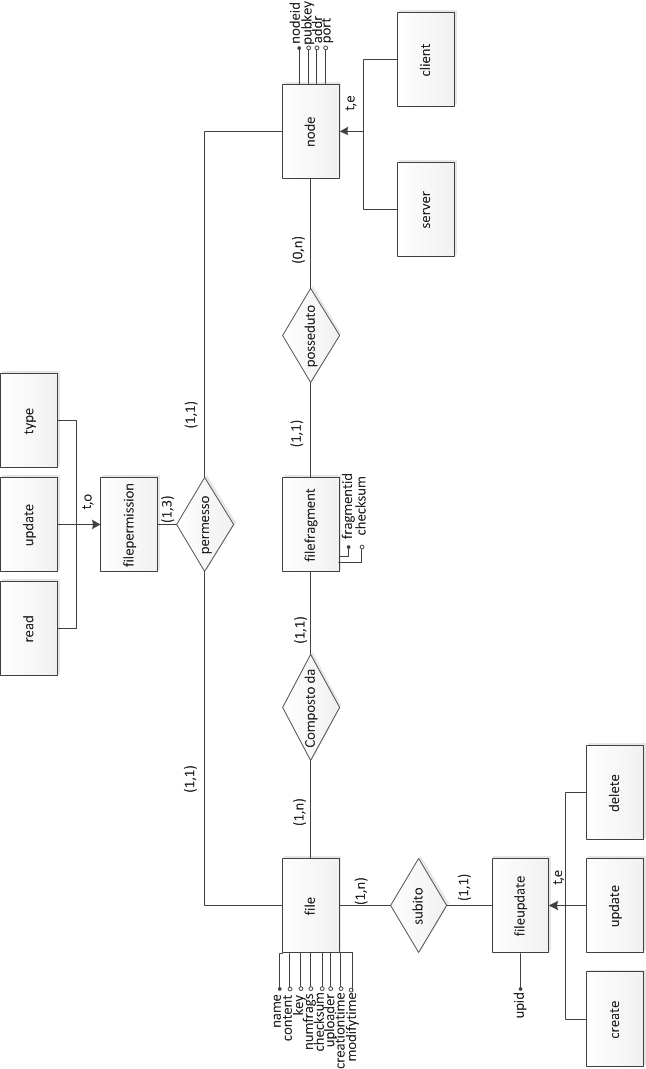
\includegraphics[width=15.3cm]{img/classdiagram.png}
\end{center}
\caption{Class Diagram}
\label{Class Diagram}
\end{figure}
In Darkcloud si fa largo uso di database\cite{database}. I dati mantenuti sul nodo sono molti. Infatti le informazioni sui dati e sugli altri nodi non sono centralizzate o mantenute in remoto, ma sono invece tutte salvate in locale. Ogni nodo, sia client che server, possiede nella cartella principale del programma un database che si chiama darkcloud.db .
Le tabelle principali che contiene sono :
\begin{itemize}
	\item FILE
	\item FILEFRAGMENT
	\item FILEPERMISSION
	\item FILEUPDATE
	\item NODE
	\item NODETYPE
	\item PERMISSIONTYPE
	\item UPDATETYPE
\end{itemize}
Lo schema relaziona del database � riportato di seguito:\\ \\
FILE(\underline{NAME},CONTENT,KEY,CHECKSUM,UPLOADER,CREATIONTIME,\\MODIFYTIME,MODIFYBY)\\
NODETYPE(\underline{NODETYPEID},NODETYPESTR)\\
UPDATETYPE(UPDATETYPEID,UPDATETYPESTR)\\
FILEFRAGMENT(\underline{NAME,FRAGMENTID},CHECKSUM,NODEID)

		\textbf{FK:} NODEID \textbf{REFERENCES} NODE(NODEID)
		
		\textbf{FK:} UPDTYPE \textbf{REFERENCES} UPDATETYPE(UPDATETYPEID)\\
FILEUPDATE(\underline{UPDID},FILENAME,NODEID,UPDTYPE,UPDTIME)

		\textbf{FK:} FILENAME \textbf{REFERENCES} FILE(NAME)
		
		\textbf{FK:} UPDTYPE \textbf{REFERENCES} UPDATETYPE(UPDATETYPEID)\\
NODE(\underline{NODEID},PUBKEY,TYPE,ADDR,PORT)

		\textbf{FK:} TYPE \textbf{REFERENCES} NODETYPE(NODETYPEID)\\
PERMISSIONTYPE(\underline{PERMTYPEID},PERMTYPESTR)\\
FILEPERMISSION(\underline{NODEID,FILENAME},PERM)

		\textbf{FK:} NODEID \textbf{REFERENCES} NODE(NODEID)

		\textbf{FK:} FILENAME \textbf{REFERENCES} FILE(NAME)

		\textbf{FK:} PERM \textbf{REFERENCES} PERMISSION(PERMID)\\
\\
All'interno del codice gli inserimenti e le letture di dati sono frequenti, invece che elencarle qui si preferisce inserirle nelle descrizioni dei comandi riportati di seguito.
\section{Crittografia}
Questo programma fa della crittografia dei dati uno dei suoi punti di forza. Dato che informazioni preziose, che potrebbero essere utilizzare per risalire ai dati, sono salvate in locale si fa un largo uso di tecniche di cifratura. In questo progetto si usano due tipi di cifratura la AES e la RSA. Sono due tipi di cifratura diversi, il primo � simmetrico, il secondo asimmetrico.
L'AES\cite{aes} (Advanced Encryption Standard) conosciuto anche come Rijndael, � l'algoritmo di cifratura a blocchi utilizzata come standard dal governo degli Stati Uniti d'America\cite{federal}. E' una tecnica di cifratura che perfino l'NSA utilizza per cifrare i documenti TOP SECRET. Questa tecnica di cifratura pu� utilizzare chiavi con lunghezza variabile di 128,192 o 256 bit e lavora con blocchi di dimensione prefissata di 128 bit. La dimensione maggiore della chiave crittografica garantisce una maggior sicurezza. Sono stati fatti dei test nel 2011 per vedere in quanto tempo con due gpu e un metodo di forza bruta si riuscisse a decifrare un file criptato in AES a 256 bit. Il risultato � stato che ci sarebbero voluti circa 13 anni di calcoli. All'interno del nostro programma per una maggior sicurezza infatti usiamo una chiave da 256bit. 

Della cifratura asimmetrica si � gi� accennato nel capitolo due, il meccanismo � semplice, ogni nodo ha una chiave pubblica e una privata, quella pubblica � scambiata con tutti i nodi e quella privata � mantenuta segreta. Se si cripta un file usando quella pubblica solo quella privata pu� decifrarlo , in questo modo tutti possono creare messaggi decifrabili solo da chi detiene la chiave privata. Lo standard de facto oggi si basa sulla cifratura RSA\cite{rsa}, un cifrario a chiave pubblica che permette di cifrare un messaggio sfruttando alcune propriet� elementari dei numeri primi. Questo cifrario prende il nome dalle iniziali dei matematici che nel 1976 lo crearono: Rivest, Shamir e Adleman. La loro idea fu quella di sfruttare la difficolt� di fattorizzare un numero intero. Di fatti la chiave pubblica � un numero N ottenuto moltiplicando due numeri primi molto grandi che restano segreti. Come nell'AES anche l'RSA pu� usare chiavi di grandezza variabile, e anche in questo caso pi� grandi sono, maggiore � la difficolt� in tentativi di attacchi di forza bruta. Le chiavi possono andare da una dimensione di 1024 ad un massimo di 4096 tipicamente. Spendendo un milione di euro per dotarsi di un cluster potente ci vorrebbero circa sei mesi per decriptare un messaggio criptato con RSA a 768 bit. Alcuni studiosi affermano che le chiavi a 1024 bit saranno scardinabili nel prossimo futuro\cite{rischio}. Infatti oggi la maggior parte dei sistemi usa chiavi a 1024 o 2048. Noi abbiamo deciso per tutelarci di usare chiavi a 4096 bit, che gli studiosi di crittografia credono sar� difficile poter scardinare in base alle previsioni sul futuro dell'informatica. 
La classe CryptUtil presente nel pacchetto Util di Darkcloud � quella nella quale abbiamo inserito i metodi che gestiscono la cifratura. Infatti vi troviamo il metodo generateKeyPair che permette di generare una coppia di chiavi RSA a 4096 bit, il metodo generateSymmetricKey che genera chiavi AES simmetriche da 256 bit, i metodi storePublicKey e storePrivateKey che permettono di memorizzare nei file usati come keystore le chiavi, i metodi getPrivateKey e getPublicKey che specifiando un file restituiscono la chiave contenuta. Poi troviamo alcuni metodi che ci permettono di convertire le chiavi in oggetti diversi, per esempio le chiavi generalmente in java sono utilizzate come oggetti Key o Secretkey per� quando abbiamo bisogno di inserire chiavi in un messaggio non possiamo lasciarle in questa forma ma dobbiamo convertirle in stringhe. Questi metodi di conversione sono privKeyToString e pubKeyToString che convertono oggetti Key in stringhe, privKeyFromString e pubKeyFromString che traducono le stringhe in oggetti Key, secretKeyFromString che traduce le stringhe in oggetti SecretKey. Troviamo poi i metodi sign e verifySign che rispettivamente servono per generare e verificare le firme da allegare ai messaggi scambiati tra nodi, firme scritte con le chiavi private e che quindi possono essere decifrate tramite le chiavi pubbliche per verificare l'identit� del mittente. Gli ultimi due metodi sono encrypt e decrypt che permettono di criptare o decriptare un array di byte specificando la chiave e il metodo di cifratura. 
I file che troviamo nella cartella principale del nostro nodo che riguardano la cifratura sono fondamentalmente quattro cio� il certificato del nostro nodo ad esempio \begin{verbatim}client_1.crt\end{verbatim}, il keystore darkcloud.keystore del nostro nodo cio� il file che contiene le chiavi pubbliche degli altri nodi che conosciamo e i file private.key e public.key che sono rispettivamente la chiave privata e pubblica del nostro nodo. 

\section{Comandi}
Andremo ora ad analizzare nello specifico quali passaggi avvengono e come vengono elaborati i dati nelle esecuzione dei comandi.
I comandi principali sono PING, PUT, GET e SHARE.
\subsection{Ping}
\begin{figure}
\begin{center}
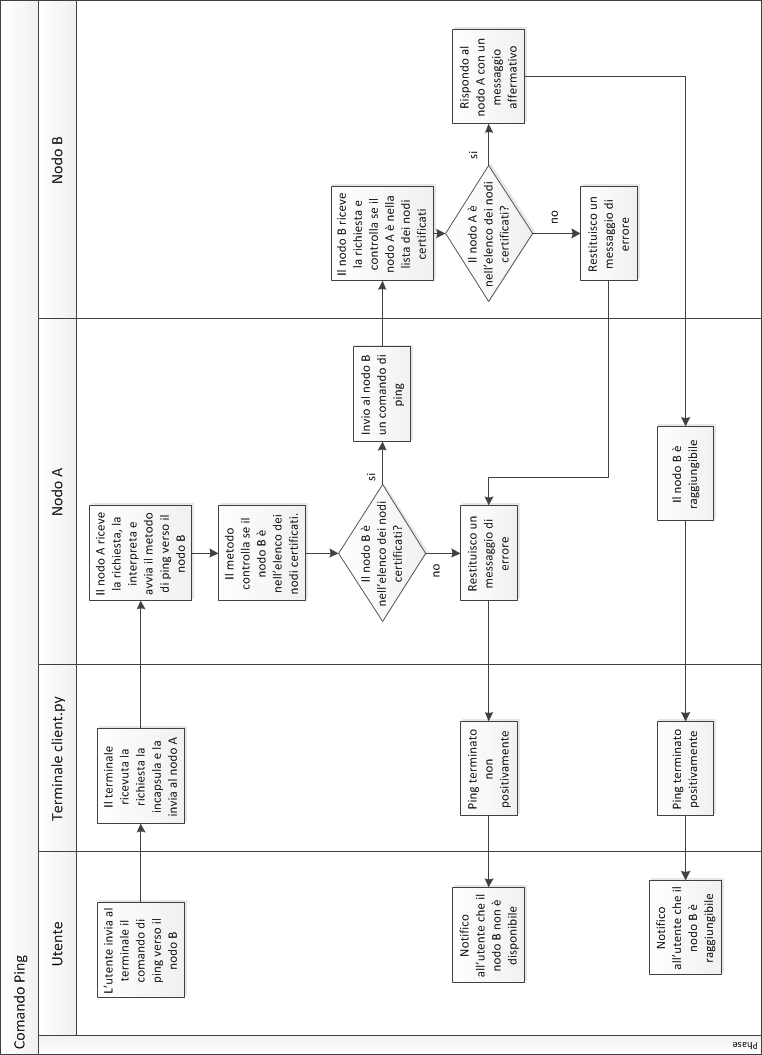
\includegraphics[width=15.3cm]{img/ping act.png}
\end{center}
\caption{Activity diagram del comando ping}
\label{Activity diagram del comando ping}
\end{figure}

Il metodo ping viene utilizzato principalmente nei terminali per verificare se un nodo client � vivo e nella classe NetPoll che lo usa per tenere aggiornato l'elenco dei server e dei client vivi sulla rete.
La sintassi del comando ping �:

python client.py -r PING -h 'indirizzo ip del client' -p 'porta di ascolto del client'

Il nodo che riceve un messaggio ha sempre in ascolto sul socket SSL la classe ClientService. Questa classe controlla continuamente se sul socket ci siano richieste. Quando ne rileva una crea una istanza della classe Client e gli passa il riferimento al socket. L'istanza di Client legge dal socket il messaggio, legge di che tipo di request si tratta e in questo caso invoca il metodo ping della classe ResponseMethods. ResponseMethods � una generalizzazione che poi viene estesa per creare ClientResponseMethods e ServerResponseMethods. L'istanza di Client passa al metodo ping la request contenuta nel messaggio. Per prima cosa il metodo ping recupera dal messaggio il campo pubkey e il campo nodeid, che contengono rispettivamente la chiave pubblica e il codice identificativo del nodo che gli ha mandato la richiesta . In seguito confrontando il nodeid con quelli salvati nelle strutture clientNodes e serverNodes controlla se � un nodo con il quale pu� dialogare e se si tratta di un server o di un client. In caso si tratti di un nodo conosciuto confronta la chiave pubblica del messaggio con quella che ha salvato nell'oggetto NetNode corrispondente, in caso sia uguale crea un nuovo oggetto response, gli da l'attributo di tipo ACK cio� di risposta positiva, e lo restituisce all'istanza di Client. L'istanza di Client ricevuto l'oggetto response lo scrive nel socket SSL, lo invia, chiude la connessione e muore.
In questa spiegazione abbiamo parlato solo della richiesta ping nel caso sia ricevuta da un nodo di tipo client, ma a differenza degli altri comandi il ping funziona nello stesso modo sia per i server che per i client. Con l'unica differenza che il client risponde anche se non viene specificata la pubkey e il nodeid, in quanto il client pu� ricevere richieste anche da terminali che di fatto non possiedono tali caratteristiche.
\subsection{Put}
\begin{figure}
\begin{center}
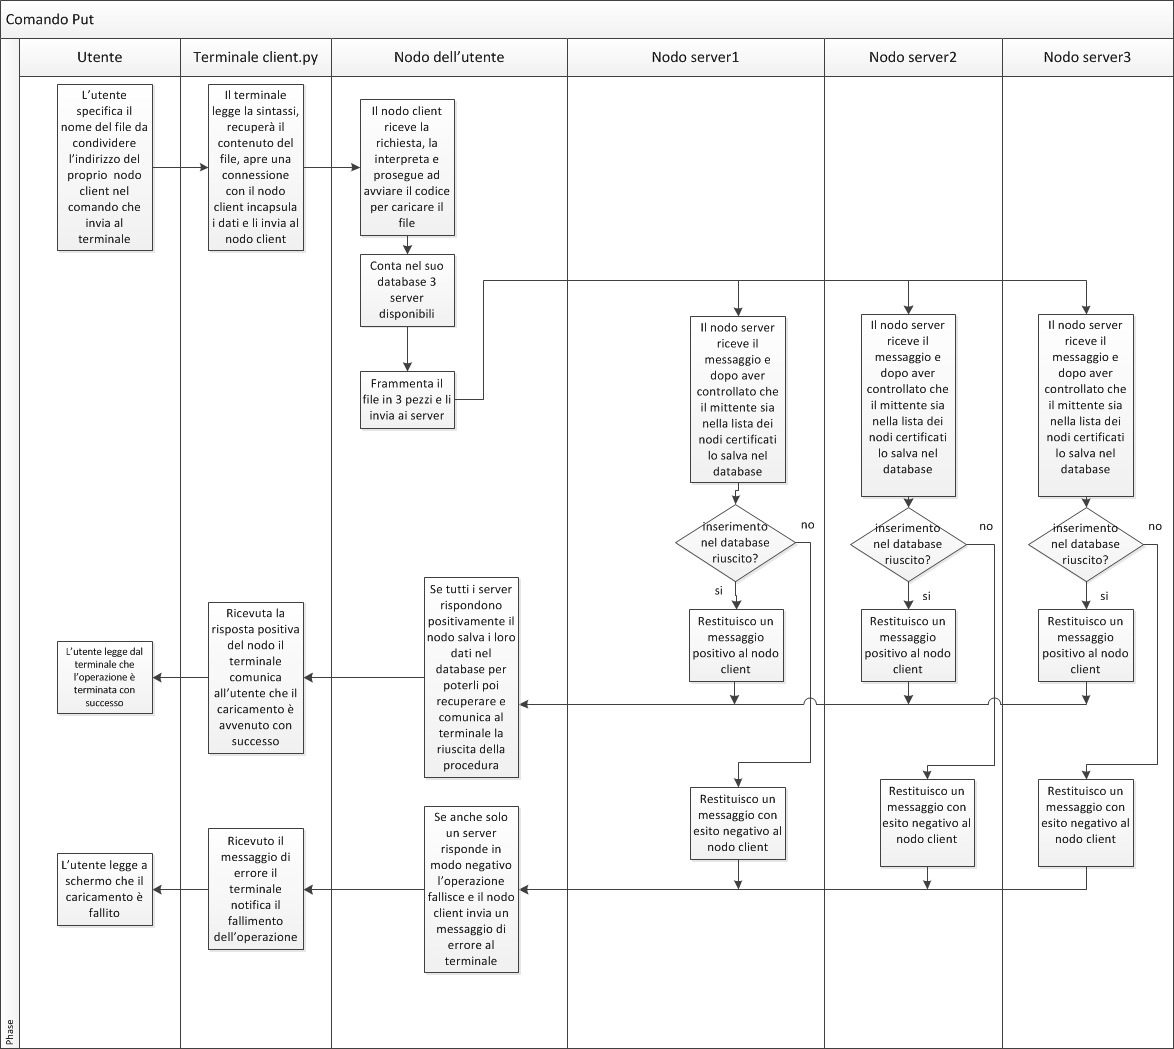
\includegraphics[width=15.3cm]{img/put act.png}
\end{center}
\caption{Activity diagram del comando put}
\label{Activity diagram del comando put}
\end{figure}

La ricezione del comando put da parte di un client invece innesca una sequenza di azioni che comprendono anche l'interazione con i server. Quindi analizzeremo sia la risposta al comando put di un client che di un server.
La sintassi del comando put �:

python client.py -r PUT -h 'indirizzo ip del client' -p 'porta di ascolto del client' -f 'nome del file locale' -F 'nome da assegnare al file in remoto'

Un utente dalla cartella dove abbiamo lo script che nei nostri test fungeva da terminale, client.py, digita il comando. In questo specifica l'ip e la porta di ascolto del client a lui dedicato, il nome di un file che si trova nella stessa cartella, o specifica prima del nome la posizione, infine il nome con il quale sar� salvato il file dal client. Premuto invio lo script cio� il nostro terminale effettua i controlli necessari sui campi inseriti, controlla se il file � codificato, in caso contario ne legge il contenuto, lo salva e calcola il checksum del file. Crea un messaggio xml, vi aggiunge i campi per il contenuto del file, il nome del file in remoto, il checksum e il tipo di codifica con cui potrebbe essere salvato il file. Dopo di ch� crea una connessione in base all'ip e alla porta di ascolto che noi abbiamo specificato e apre un socket SSL tramite il quale invia il messaggio al nostro client. Il nostro client che ha ClientService in ascolto rileva il messaggio, istanzia Client e gli passa il socket. Client legge il messaggio legge il tipo di richiesta e invoca il metodo put della classe ClientResponseMethods passandogli l'oggetto request contenuto nel messaggio.
Il metodo put di ClientResponseMethod legge dall'oggetto request il contenuto del campo file, controllando che non sia vuoto. Recupera anche il nome del file e il tipo di codifica, in caso il file risulti codificato il metodo procede a decifrarlo, dopo di che legge il campo checksum e calcola il checksum del file ricevuto. Paragona il checksum calcolato con quello del messaggio per verificare errori di trasmissione, in caso combacino procede. Ora tramite il metodo getAliveServerNodes della classe Darkcloud recupera una copia dei NetNode che sono vivi e li pone in un hashmap. Ora si rende necessario mescolare l'hashmap in modo che i server a cui si inviano i frammenti non siano tutti consecutivi. Per fare questo creiamo una seconda hashmap con la stessa struttura di quella con i server. Creiamo un array di stringhe e vi salviamo tutte  le chiavi della hashmap dei server. Usiamo la funzione Collections.shuffle(keys) per mescolarne le stringhe e con un ciclo for inseriamo nella seconda hashmap i NetNode usando come di selezione le stringhe mescolate.
A questo punto avremo la seconda hashmap che contiene i NetNode mescolati a dovere. Procediamo con la fase di cifratura del file. 
Generiamo una chiave simmetrica tramite il metodo generateSymmetricKey della classe CryptUtil. Criptiamo il contenuto del file sempre tramite un metodo di CryptUtil che si chiama encrypt. Particolare attenzione va fatta in questi passaggi in quanto nelle comunicazioni tra metodi i byte vanno passati codificati in base 64, inoltre i metodi che criptano vogliono in ingresso byte e non stringhe, maggiori dettagli vengono forniti nei prossimi paragrafi riguardanti la crittografia. 
Giunti a questo punto abbiamo il contenuto del nostro file criptato e contenuto in un array di byte.  
Per sapere quanto grandi devono essere i nostri frammenti prendiamo la dimensione del file criptato e la dividiamo per il numero di server. In questo modo per� se la divisione ha del resto andrebbero persi dei byte, quindi aggiungiamo 1 alla dimensione dei frammenti. Tramite un ciclo for andiamo a leggere porzioni del file criptato che vengono poi salvate in un array di stringhe, la lettura parziale avviene tramite la funzione substring che permette di leggere da una stringa un numero dato di caratteri a partire da una posizione a scelta. Ora le parti sono contenute nel nostro array di stringhe. In un ciclo for che si ripete per il numero di server che abbiamo andiamo ad inviare i frammenti. Creiamo prima di tutto un oggetto NetNode e gli andiamo a mettere dentro quello preso dalla hashmap mescolata, in modo da poter dopo usare il metodo send e mandargli un messaggio. Ora calcoliamo il checksum del frammento, prendiamo la request che ci ha mandato il terminale e andiamo ad aggiungergli i campi dove inseriamo il contenuto criptato, il checksum, dato che ci sono ancora i campi creati dal terminale la request contiene anche il nome del file e il nodeid del client. 
Completato l'oggetto request questo viene mandato tramite il metodo send al NetNode preso dalla hashmap mescolata. 

Ora il server riceve tramite la consueta procedura l'oggetto request di tipo put quindi viene invocato il metodo put del ServerResponseMethod. Il metodo put del server legge il contenuto del file e fa il controllo del checksum. Se il checksum corrisponde procede a salvare nel database i dettagli del frammento. I campi che vengono salvati sono nome del file, contenuto del frammento, checksum, nodeid del client, data di creazione e data di modifica. Inoltre dato che viene tenuta traccia anche delle modifiche fatte ai file viene anche inserito un nuovo record nella tabella FILEUPDATE con i dati nome del file, nodeid, tipo di update, e data della modifica. Al termine del metodo se tutto va bene si restituisce un oggetto response di tipo ACK che viene mandato al client.

Quando il client riceve il response di tipo ACK passa al salvataggio nel database dei dettagli di questo frammento nella tabbela FILEFRAGMENT, che comprendono nome del file, un intero che indica il numero del frammento, il checksum e il nodeid del server dove il frammento � salvato. Alla fine di questo ciclo for se tutti i frammento sono stati correttamente inviati il metodo prende la chiave simmetrica usata per criptare il file e la cripta usando la sua chiave pubblica. Poi registra sul database nella tabella FILE i dettagli del file appena splittato sui server, salvandone nome, chiave criptata, checksum, data di creazione e data di modifica. 
\subsection{Get}
Il comando get usato tramite un terminale permette di recuperare un file precedentemente salvato. Come per il comando put questo comando fa eseguire codice diverso a seconda se sia inviato ad un client o ad un server. Nel seguito analizzeremo entrambi.
La sintassi del comando get �:

python client.py -r GET -h 'indirizzo ip del client' -p 'porta di ascolto del client' -F 'nome del file in remoto'

Quando un utente vuole recuperare un file che ha salvato in darkcloud sar� sufficiente che usi il comando get, il codice che ci sta dietro recuperer� i frammenti, decripter� il contenuto e dar� in uscita il contenuto del file. Ma procediamo a vedere nei dettagli cosa accade nel codice.
Il terminale come nel caso del ping e del put creer� un messaggio xml e al suo interno metter� il nome del file da recuperare, i dati del nodo client che intende usare per recuperarlo. Dopo di che creer� un socket SSL e invier� al nodo client che voi avete specificato, e che � l'unico che un utente deve usare per recuperare i suoi file, il messaggio. Il ClientService sempre in ascolto rilever� il messaggio, creer� in istanza di Client e gli passer� il socket. Client legger� il messaggio, recuperer� il tipo di request contenuta al suo interno e invocher� il metodo corrispondente del ClientResponseMethods, nel nostro caso il metodo get.
Il metodo prende in ingresso un oggetto request, e inizia leggendo il campo file e verificando che non sia vuoto. Poi passa a leggere all'interno del campo file l'attributo name,cio� il nome del file, e controlla che anche esso non sia nullo. Fatti tali controlli il metodo fa un join sulle tabelle FILE e FILEFRAGMENT sulla colonna name, dove il valore name � uguale al nome passato nella request. Leggendo poi in tale ordine la chiave di decriptazione, il fragmentid cio� il numero del frammento, il checksum del frammento e il nodeid dove il frammento � salvato. Ordinando i risultati per fragmentid. Se la query restituisce risultati il passo successivo � decriptare la chiave. Tramite il metodo decrypt della classe Cryptutil specificando la chiave da decriptare, la propria chiave privata recuperata tramite il metodo getPrivateKey di Darkcloud e infine il tipo di cifratura nel caso RSA, otterremo la chiave simmetrica del file in chiaro sotto forma di stringa. Visto che per� per decifrare il file tramite il metodo decrypt dopo averlo ricomposto dovremo specificare la chiave sotto forma di oggetto Secretkey, la convertiamo subito da stringa a Secretkey tramite il metodo secretKeyFromString della classe CryptUtil. A questo punto tramite un ciclo for andiamo a ripetere le prossime operazioni per il numero di record restituiti dal join. Prendiamo il primo nodeid restituito dal join e copiamo l'oggetto NetNode che gli corrisponde in una istanza locale. Possiamo farlo tramite il metodo getAliveServerNodes().get(nodeid). Ora abbiamo il NetNode pronto per quando dovremo inviare una request al server. Creiamo un oggetto request, impostiamo l'attributo tipo come get e gli aggiungiamo un nuovo campo nominandolo file, al quale poi aggiungiamo l'attributo name. Attribuiamo a name il nome del file ed inviamo al server questa request tramite il metodo send dell'oggetto NetNode che abbiamo prima recuperato. 

Ora il server ricever� la nostra richiesta, legger� dall'attributo name del campo field dell'oggetto request il nome del file. Tramite una select sulla sua tabella FILE, in base al nome recuperer� i seguenti campi: contenuto, checksum, data di creazione, data di modifica, il nodeid del nodo uploader e la modificabilit�. Avendo tutti i dati necessari ora il metodo get creer� un nuovo oggetto response, impostanto l'attributo tipo su ACK. A questo response aggiunge un campo file e a questo campo aggiunge gli attributi checksum, data creazione, data modifica, uploader, modificabilit� e contenuto del file. Assegna a questi attributi i valori letti nel database e restituisce questo oggetto response al client.

Il client se la response � di tipo ACK procede alla lettura del campo file. Come prima cosa legge l'attributo checksum e lo paragona con quello che calcola dal frammento contenuto nell'oggetto response. Se combaciano aggiunge il frammento del file alla stringa fileContent. La stringa fileContent alla fine del ciclo for contiene tutto il file cifrato ricomposto. Quindi � pronta per essere decriptata tramite la chiave che all'inizio del metodo avevamo recuperato dal database. Decifrato il file sar� sufficiente inserirlo nell'oggetto response e restituirlo al terminale. Ora il terminale ha il file richiesto dall'utente. Lo script che abbiamo usato per i test stampa direttamente a schermo il contenuto, se vogliamo ottenere il file baster� indirizzare il risultato del comando in un file con quel nome.
\subsection{Share}
Il comando share permette di condividere la conoscenza di un determinato file con altri utenti. Come abbiamo visto nel comando put, quando un client salva in darkcloud un file questo viene spezzettato ed inviato ai server, dopo di che il client salva i dati necessari a ricomporlo in sicurezza. Per far si che anche un altro client possa recuperare quel file dobbiamo prendere i dati contenuti nel database del client che condivide e copiarli nel database del client con cui vogliamo condividere il file.
Quindi a differenza degli altri comandi che vedevano coinvolti un client e diversi server questa volta nel codice del comando share devono interagire due client. nel caso del put e del get avevamo la versione del comando per il client e quella per il server, questa volta invece il codice del comando share � contenuta solo nei metodi di risposta del client, cio� nella classe ClientResponseMethod. Per� visto che la procedura di salvataggio deve essere fatta direttamente dal nodo ricevente, abbiamo creato un altro metodo, che si chiama receive. Un nodo non pu� salvare informazioni direttamente sul database di un altro nodo, sarebbe pessimo per la sicurezza. Quindi quando noi invochiamo il comando share dal nodo A verso il nodo B per condividere un file, il nodo A reperisce nel suo database le informazioni del file, e le invia al metodo receive del nodo B, che procede con il controllo dei dati e il salvataggio nel suo database.
La sintassi del comando � :

python client.py -r SHARE -h 'ip del client che condivide' -p 'porta del client che condivide' -F 'nome del file remoto' -H 'ip del ricevente' -P 'porta del ricevente'

Quando un utente vuole condividere con un altro la conoscenze di un file utilizza il suo terminale e il comando sopra scritto. Quando il terminale invia il messaggio al client, questo lo riceve tramite la classe ClientService e crea un istanza della classe CLient, la quale tradurr� il messaggio in un oggetto request. Riconosciuto che  l'oggetto request � di tipo share proceder� ad invocare tale metodo passandogli i campi contenuti nel messaggio. Il metodo share procede al controllo dell'esistenza del campo sharing. Nel campo sharing sono contenuti tre attributi, secondhost, secondport e remotefile. Questi attributi sono stati attribuiti dal terminale con i campi specificati nella sintassi del comando share. Il codice prosegue controllando che a tutti gli attributi sia stato assegnato un valore. Fatto ci� si passa a leggere dal database i dati che riguardano il file. Dobbiamo prendere i file da due tabelle, FILE e FILEFRAGMENT. Per fare questo facciamo un join sul'attributo name che deve essere uguale al nome del file remoto specificato nel comando. I risultati verranno ordinati per fragmentid e i campi selezionati sono in ordine la chiave del file, il checksum del file intero, la data di creazione del file, il numero che identifica il frammento, il checksum del frammento e nodeid del server che conserva il frammento. 
Si passa ora a recuperare il NetNode corrispondente al client a cui dobbiamo inviare i dati. I NetNode sono identificati da un codice alfanumerico ottenibile dalla funzione getNodeKey della classe Darkcloud dando in ingresso l'indirizzo ip e la porta di ascolto del nodo. Ottenuto il nodeid possiamo procedere a copiare in locale l'oggetto NetNode del client a cui dobbiamo inviare i dati. Per ottenere questo oggetto usiamo il metodo Darkcloud.getIstance().getAliveClientNodes().get(nodeid) .
Come notate stiamo prendendo il NetNode dalla struttura dati dove sono salvati quelli segnati come vivi. Infatti anche i client proprio come i nodi server vengono contattati periodicamente per verificare che siano online. Il prossimo passo consiste nel preparare la chiave del file per il trasferimento. Quando noi abbiamo salvato la chiave simmetrica del file, nel metodo put, la abbiamo criptata con la nostra chiave pubblica. Ora dobbiamo decriptarla, con la nostra chiave privata e criptarla con la chiave pubblica del nodo a cui dobbiamo mandarla. Per decriptarla usiamo il metodo decrypt della classe Cryptutil, dandogli in ingresso la stringa che abbiamo preso nel database, la nostra chiave pubblica ottenibile con il metodo Darkcloud.getIstance().getPrivateKey(), e infine specificando il metodo di decriptazione cio� RSA. Il metodo decrypt ci restituisce un array di byte, che noi convertiamo in un oggetto SecretKey tramite il metodo della Cryptutil denominato secretKeyFromString. Questo passaggio � necessario in quanto il metodo per criptare accetta in ingresso come chiave solo un oggetto SecretKey. La chiave pubblica del nodo ricevente � salvata nel NetNode corrispondente che abbiamo recuperato, e per usarla baster� il metodo NetNode.getPubKey(). Fornendo la chiave simmetrica decriptata e la chiave pubblica del nodo ricevente al metodo encrypt otteniamo la chiave simmetrica criptata pronta per essere spedita. Ricordo che le stringhe passate tra i metodi e inserite nei messaggi devono essere codificate in base64 per evitare problemi di trasferimento. Ora dobbiamo preparare un oggetto request e inserirgli i valori da mandare al client ricevente. L'oggetto request � di tipo receive, ai nostri oggetti request o response possiamo aggiungere tutti i campi che vogliamo e nei campi possiamo inserire tutti gli attributi che vogliamo. In questo caso dobbiamo trasferire un insieme di informazioni che riguardano il file intero e un numero variabile di insiemi di informazioni che riguardano i frammenti. Per questo prima creiamo l'oggetto request, impostiamo il tipo come receive, vi creiamo un nuovo campo che chiameremo file nel quale andiamo ad inserire gli attributi che riguardano il file intero, che sono nome, chiave simmetrica, checksum, data di creazione e numero di frammenti. Ora, tramite un ciclo for che si ripete tante volte quanti sono i frammenti, andiamo a creare tanti campi quanti frammenti. Ogni campo si chiamer� fragment'i', dove i � il numero che identifica il frammento. Tramite il ciclo in ognuno di questi campi inseriremo come attributi i dati dei frammenti, che sono numero del frammento, checksum e l'identificativo nodeid del server dove si trova. Terminata la preparazione della request possiamo mandarla al client ricevente. Usiamo il metodo send dell'oggetto NetNode precedentemente recuperato. 
Il metodo send aprir� un socket SSL con l'altro client, e invier� il messaggio.

Il client ricevente tramite ClientService riceve il messaggio, crea un istanza di Client, la quale riconosce il tipo di request come receive. Invoca il metodo receive dalla classe ClientResponseMethod e gli passa la request.
Il metodo receive legge per primo l'attributo del campo file che contiene il numero dei frammenti. Poi imposta un ciclo for che legge i campi che contengono i dati dei frammenti e li salva nella tabella FILEFRAGMENT. Se tutti i frammenti vengono salvati il metodo receive procede con la lettura del campo file e salva nella tabella FILE i dati in esso contenuto. Se questi inserimenti avvengono con successo il metodo receive crea un oggetto response e gli attribuisce il tipo ACK che indica la corretta fine del metodo. Restituisce poi questa response al metodo Client che provveder� ad inviarla al client che ha fornito i dati.

Il client che ha inviato i dati riceve cosi la response positiva, e procede a sua volta a notificare al terminale che l'operazione � terminata con successo. Per farlo crea una response di tipo ACK e la restituisce al terminale tramite la classe Client. Il terminale da cui era partito il comando, in caso di ricezione del messaggio ACK stampa a schermo un messaggio che ci informa che il file � stato condiviso con il client specificato. 
\section{File di log}
Una cosa essenziale in ogni software � il file di log, tramite questo possiamo controllare il funzionamento del nostro nodo e verificare la presenza di errori o anomalie. In caso di errori possiamo verificare dove si sono verificati questi errori all'interno del software e da cosa sono stati scatenati. Maggiore � l'accuratezza e maggiori sono i dettagli riportati in un file di log maggiore sar� la velocit� con la quale si capir� il problema e minore il tempo impiegato per risolverlo. Proprio per questo abbiamo utilizzato all'interno del nostro software un sistema di log molto articolato. Per farlo utilizziamo la classe Logger che fa parte del package org.apache.log4j . 
Log4j � un progetto Open Source dell�Apache Software Foundation (ASF) che permette di monitorare un�applicazione Java durante il suo utilizzo qualora non fosse possibile utilizzare strumenti di debugging, si pensi ad esempio quando una applicazione � distribuita sul web o � di tipo multithreading. Il logging ha per� una controindicazione: porta ad un decremento delle performance. Per alleviare questo difetto, log4j � stato sviluppato per essere veloce ed estendibile, permettendo vari livelli di granularit� nel controllo del logging. Il vantaggio pi� importante che ha un sistema di logging ha rispetto a riempire il nostro codice di System.out.println, � che � possibile controllare quando visualizzare gli statement di log. In altre parole � possibile dividere lo spazio dei log, che � lo spazio dove risiedono tutti gli statement di log, in categorie definite da criteri decisi dallo sviluppatore. La classe Logger rappresenta appunto uno spazio dei log che rispetta dei determinati criteri.
Infatti nella cartella principale del nostro nodo troviamo il dile darkcloud.log che contiene tutte le informazioni di cui nel codice abbiamo deciso di tener traccia. Sono divise in categorie quali Message, Config, Info ed Error. Inoltre in tali file di log vengono indirizzati i messaggi di errore che il sofware genera. 
Per ogni errore o per capire meglio il funzionamento del programma si invita l'utilizzatore a leggere il file di log.















\chapter{Risultati sperimentali}
Al termine della fase di programmazione il programma Darkcloud risulta pienamente funzionante. Solitamente durante lo sviluppo di un software per verificarne il funzionamento e testare la funzionalit� dei comandi si fanno continui test sulle macchine degli sviluppatori e su altre architetture. Anche nel nostro caso abbiamo svolto diversi test nella fase di development. Giunti ad avere un software funzionante un modo per testarne la qualit� � effettuare dei test sulle prestazioni. I test di prestazioni sui software possono essere di diversi tipi, noi abbiamo effettuati alcuni test sulla velocit� e sul carico di lavoro.
Sapere se la velocit� di esecuzione di un comando � compatibile con i tempi di utilizzo normali � importante, in quanto se andassero a rallentare quello che � il lavoro dell'utilizzatore ultimo sarebbe controproducente. Oggi se un computer � troppo lento o un programma impiega troppo tempo, e come nel nostro caso l'utilizzatore � un professionista che ha bisogno di efficienza nel lavoro, questo ultimo non ci penser� due volte a cambiare prodotto. Un altro parametro importante � il carico di lavoro, cio� la fatica che il computer fa per per eseguire un certo comando. E' vero che oggi i computer sono molto potenti, ma l'aumento della portabilit� dei dispositivi porter� anche a riduzioni della potenza di calcolo. Per quanto riguarda la compatibilit� su diverse piattaforme e sistemi operativi il nostro programma � molto avvantaggiato, in quanto � scritto in java. Java � un linguaggio indipendente dalla piattaforma, infatti i programmi scritti in linguaggio Java sono destinati all'esecuzione sulla piattaforma Java, ovvero saranno lanciati su una Java Virtual Machine e, a tempo di esecuzione, avranno accesso alle API della libreria standard. Ci� fornisce un livello di astrazione che permette alle applicazioni di essere interamente indipendenti dal sistema su cui esse saranno eseguite.

I nostri test sono stati effettuati principalmente su due sistemi. Il personal computer del tesista,che chiameremo calcolatore A, e il server universitario Capoeira.
Le configurazioni hardware dei due sistemi sono molto differenti. Le componenti che faranno la differenza nelle prestazioni sono la cpu, la memoria e il disco fisso.
Il calcolatore A ha una cpu Intel i5-750, un modulo di memoria ram da 4gb e disco rigido ssd. Il server Capoeira ha 2 cpu Intel E5540, 16gb di memoria ram e dischi scsi a 15000 rpm. La differenza che pi� sentiremo nei test riguarda i processori, infatti il server ha una capacit� di calcolo superiore di quasi due volte a quella del calcolatore A. Il processore intel i5-750 infatti ha quattro core mentre ogni singolo E5540 ha quattro core, moltiplicato per due processori fa 8 core. Il calcolatore A ha per� i core con frequenza fissa a 3.6 ghz mentre quelli di capoeira hanno una frequenza che varia in base alla richiesta.
Il sistema operativo sul calcolatore A � Windows 7 64bit sul quale tramite VirtualBox � stato usato in macchina virtuale il sistema operativo Debian 4.3.5 basato sul kernel linux 2.6.32. Si � optato per questa soluzione per semplificare l'utilizzo degli strumenti di sviluppo e test. Il server Capoeira invece ha installato Debian 4.5.3 basato sul kernel linux 3.0.0. 

Per misurare i tempi impiegati dai comandi dall'avvio al termine dell'esecuzione si � impiegato il programma linux TIME. Questo comando anteposto ad un altro restituisce alla fine dell'esecuzione il tempo totale impiegato dal processo e la percentuale di cpu utilizzata per eseguirlo. 
I comandi utilizzabili al momento sono il ping, il put, il get e lo share. Il ping � un comando usato solo per verificare la disponibilit� in rete di una macchina, quindi su di esso non sono stati fatti test prestazionali. Sono invece stati testati il put, il get e lo share. Un esempio di sintassi del test � il seguente
\begin{verbatim}time python client.py -r PUT -h 127.0.0.1 -p 18100 -f prova.txt 
-F prova.txt\end{verbatim}\\
I test sono stati fatti tutti creando i nodi in locale quindi non tengono conto di eventuali ritardi dovuti a latenze della rete. Il fattore delle latenze di rete non �  
quantificabile a priori, senza conoscere i casi di uso specifici, quindi per il momento � stato ignorato. Facendo test in locale possiamo capire come reagisce il software quando le istanze aumentano e il carico dei dati si incrementa. Possiamo dire che l'obbiettivo dei nostri test � capire se il software gestisce bene l'aumento dei nodi, che comporta a seconda del comando un aumento della complessit� dell'architettura e ci permette di valutare la scalabilit� del programma. 

Per testare il put abbiamo creato in locale una architettura che comprendeva un nodo client e cinque nodi server. Si � iniziato con l'invio di un file ad un solo server, poi verso due server incrementando il numero fino all'invio a cinque server. Per ogni caso la misurazione � stata eseguita dieci volte e al termine raccolti i risultati abbiamo fatto la media. Il file inviato era sempre della stessa dimensione, cio� 1KB, in modo da uniformare i risultati. In questo test l'aumento del numero dei server comporta un aumento del codice che il client deve eseguire, osservare i tempi e i carichi ci dir� se il software � in grado di incrementare le proprie prestazioni o se ci sono colli di bottiglia che rallentano.

Ecco di seguito i test sul put.
\begin{table}[htbp]
\begin{center}
\begin{tabular}{|c|c|c|}
\hline
n�server & tempo di esecuzione & uso cpu\\
\hline
1 & 1,2 sec & 3\%\\
\hline
2 & 1,9 sec & 2\%\\
\hline
3 & 2,6 sec & 1\%\\
\hline
4 & 3,3 sec & 1\%\\
\hline
5 & 4 sec & 1\%\\
\hline
\end{tabular}
\end{center}
\caption{Test su Capoeira del comando PUT}
\label{tab:table}
\end{table}
\begin{table}[htbp]
\begin{center}
\begin{tabular}{|c|c|c|}
\hline
n�server & tempo di esecuzione & uso cpu\\
\hline
1 & 1,8 sec & 1\%\\
\hline
2 & 2,8 sec & 1\%\\
\hline
3 & 4,1 sec & 1\%\\
\hline
4 & 5,7 sec & 1\%\\
\hline
5 & 6,1 sec & 1\%\\
\hline
\end{tabular}
\end{center}
\caption{Test sul calcolatore A del comando PUT}
\label{tab:table}
\end{table}

I test eseguiti sul comando get vanno invece a testare il tempo di risposta e il carico di lavoro a cui si sottopone la cpu quando si devono recuperare dai server le informazioni per ricomporre il file. Anche in questo caso abbiamo utilizzato file di dimensione uguale, tutti di 1KB. Il programma utilizzato � stato time con una sintassi simile alla seguente:
\begin{verbatim}time python client.py -r GET -h 127.0.0.1 -p 18100 -F prova.txt\end{verbatim}\\
Come nel get per testare la scalabilit� del software nell'aumento della difficolt� computazionale abbiamo incrementato gradualmente i nodi dai quali andavamo a prelevare l'informazione. In questo modo il programma deve eseguire pi� comandi. Prima abbiamo recuperato dal nostro client un file contenuto su un nodo, poi su due nodi incrementando fino a cinque nodi. Per ognuna di queste architetture si sono fatti dieci rilevamenti e i valori in tabella ne sono le medie. Si riportano di seguito le tabelle dei risultati dei test del get.
\begin{table}[htbp]
\begin{center}
\begin{tabular}{|c|c|c|}
\hline
n�server & tempo di esecuzione & uso cpu\\
\hline
1 & 1,4 sec & 3\%\\
\hline
2 & 2,1 sec & 2\%\\
\hline
3 & 2,3 sec & 2\%\\
\hline
4 & 2,8 sec & 1\%\\
\hline
5 & 3,6 sec & 1\%\\
\hline
\end{tabular}
\end{center}
\caption{Test su Capoeira del comando GET}
\label{tab:table}
\end{table}
\begin{table}[htbp]
\begin{center}
\begin{tabular}{|c|c|c|}
\hline
n�server & tempo di esecuzione & uso cpu\\
\hline
1 & 2,1 sec & 1\%\\
\hline
2 & 3,0 sec & 1\%\\
\hline
3 & 3,6 sec & 1\%\\
\hline
4 & 4,2 sec & 1\%\\
\hline
5 & 6,5 sec & 2\%\\
\hline
\end{tabular}
\end{center}
\caption{Test sul calcolatore A del comando GET}
\label{tab:table}
\end{table}
L'ultimo comando da analizzare � lo share, a differenza del put e del get questo comando non fa interagire nodi client con nodi server, ma solo nodi client tra di loro. Quindi nei test di questo comando non sarebbe utile ai fini dell'analisi della scalabilit� l'aumento del numero dei server, ma piuttosto l'aumento del numero dei client con cui un nodo client voglia condividere un informazione. Per questo motivo in questi test abbiamo utilizzato il comando share con un numero sempre maggiore di client come obbiettivo, prima con un solo client poi con due crescendo fino a cinque client. Per fare questo abbiamo incontrato il problema che lo share accetta solo un altro client come destinatario dello share. Per ovviare questo problema abbiamo realizzato uno script shell all'interno del quale abbiamo scritto tanti comandi share concanetati dall'operatore \& che nella console permette di eseguire i comandi in background. In questo modo abbiamo inviato contemporaneamente le richieste di share e le abbiamo fatte processare tutte contemporaneamente. Usando poi il programma time seguito dallo script abbiamo ottenuto il tempo totale dell'esecuzione dei comandi share. La sintassi del file script.sh per lo share delle informazioni di un file da un nodo verso altri due per esempio sarebbe
\begin{verbatim}python client -r SHARE -h 127.0.0.1 -p 18100 -F prova.txt -H 127.0.0.1 
-P 18101 & python client -r SHARE -h 127.0.0.1 -p 18100 -F prova.txt 
-H 127.0.0.1 -P 18101\end{verbatim}\\
Mentre invece la sintassi del comando time con lo script �
\begin{verbatim}time ./script.sh\end{verbatim}\\
Per ogni architettura di prova sono stati eseguiti dieci test e il valore riportato in tabella rappresenta la media. Il file condiviso era situato su un solo server in modo da poter focalizzare i test sulla scalabilit� dello share e non della dimensione dei dati salvati, inoltre tale file era delle dimensioni di 1KB. Si riportano di seguito le tabelle dei test dello share.
\begin{table}[htbp]
\begin{center}
\begin{tabular}{|c|c|c|}
\hline
n�client & tempo di esecuzione & uso cpu\\
\hline
1 & 1,4 sec & 3\%\\
\hline
2 & 1,5 sec & 3\%\\
\hline
3 & 1,6 sec & 7\%\\
\hline
4 & 1,7 sec & 8\%\\
\hline
5 & 2,2 sec & 8\%\\
\hline
\end{tabular}
\end{center}
\caption{Test su Capoeira del comando SHARE}
\label{tab:table}
\end{table}
\begin{table}[htbp]
\begin{center}
\begin{tabular}{|c|c|c|}
\hline
n�client & tempo di esecuzione & uso cpu\\
\hline
1 & 1,9 sec & 1\%\\
\hline
2 & 2,5 sec & 1\%\\
\hline
3 & 3,6 sec & 1\%\\
\hline
4 & 4,2 sec & 1\%\\
\hline
5 & 7 sec & 1\%\\
\hline
\end{tabular}
\end{center}
\caption{Test sul calcolatore A del comando SHARE}
\label{tab:table}
\end{table}\\
Ad una prima analisi i risultati potrebbero sembrare strani visto che su Capoeira l'utilizzo della cpu aumenta mentre sul calcolatore A rimane basso. Questi valori sono dovuti al tipo di processori usati. Infatti il calcolatore A ha un processore da desktop con frequenza molto alta, risparmi energetici disattivati e alto consumo quindi ha il processore sempre ad un regime di lavoro alto. I processori dei server sono pi� dinamici dovendo pensare anche al consumo dato che sono in numero molto maggiore. La potenza data dall'utilizzo di 8 core nel server per� si nota dai tempi molto pi� bassi. I risultati sono positivi anche per quanto riguarda la scalabilit� in quanto l'aumento dei tempi � lineare e questo indica che il software gestisce bene l'incremento di complessit� computazionale. 
\chapter{Conclusioni}
\section{Sviluppi futuri}
Nonostante il programma sia pienamente funzionante, e i nodi server possano gi� essere installati su sistemi operativi virtuali situati su piattaforme di cloud computing, il progetto iniziale prevede che il software sia ottimizzato per il cloud computing. Come avevamo accennato al termine del capitolo 2 esistono servizi cloud di tre livelli: IaaS quindi hardware remoto, PaaS cio� piattaforme remote e SaaS cio� software remoto. Al momento Darkcloud pu� essere usato su servizi cloud di hardware e piattaforma remoti. Il prossimo passo sar� verso l'utilizzo di un livello ancora pi� alto, cio� SaaS. Se si utilizza un servizio per avere direttamente un software funzionante in remoto invece che dover realizzare un sistema operativo o una piattaforma sulla quale far girare il nostro software si sprecheranno meno risorse e questo comporter� un costo minore delle istanze server di Darkcloud, potendo aumentarne cosi il numero a favore della sicurezza. Avere software ottimizzato ed eseguito su sistemi pi� embedded che general purpose rende pi� sicuri i nostri dati e i nostri nodi server. Ogni provider di cloud ha librerie diverse per ottimizzate l'esecuzione del codice sui suoi sistemi. 

Quindi per poter utilizzare servizi cloud a livello SaaS bisogner� studiarne le librerie e andarle ad inserire nel codice per realizzare versioni di Darkcloud ad hoc per i nodi server. Dato che era prevista questa evoluzione il software � stato strutturato in modo da rendere semplice l'implementazione di nuove librerie. 

Dato che si potr� cosi sviluppare una architettura ancora pi� solida e complessa con l'utilizzo di vari servizi cloud si potrebbe anche introdurre un algoritmo di replicazione parziale dei dati in modo da avere una ridondanza dei dati su pi� servizi. Questo potrebbe garantire non solo una maggior garanzia sulla segretezza dei propri dati, ma anche una maggior reperibilit� dei dati. Non dovendo temere l'eventualit� di disservizi da parte di alcuni provider di cloud. 

Al momento quando il un dato viene trasmesso o ricevuto vengono fatti dei controlli per testare l'eventuale presenza di errori nel dato. Questi controlli si basano sul checksum e possono garantire solo l'integrit� del dato. Un interessante apporto al software potrebbe essere dato dall'introduzione di un algoritmo di correzione degli errori. Esistono infatti algoritmi che trasmettendo i dati in frammenti, in caso di perdita di un frammento, sono in grado di ricostruirlo in base agli altri.

Oltre ad adattare Darkcloud a vari servizi cloud uno sviluppo futuro potrebbe riguardare la realizzazione di terminali. Con terminali si intende software di interfaccia tra la rete Darkcloud e l'utente, che al momento � svolto dal nostro script python client.py. L'unico limite allo sviluppo dei terminali � la fantasia, si potrebbe realizzare interfacce su pagine web, software per personal computer, applicazioni per tablet smartphone e cellulari. Dato che questo software � stato realizzato puntando alla sicurezza dei dati, vogliamo ricordare ai futuri sviluppatori di terminali di tenere sempre presente questo, in modo da rinforzare la sicurezza nel punto pi� vulnerabile delle moderne tecnologie di rete che � vicino all'utente utilizzatore, che nella maggior parte dei casi � il meno esperto.

\section{Considerazioni finali}
Questa tesi ha voluto analizzare la nascita del progetto Darkcloud, il tesista ha assistito l'ingegner Fabio Manganiello e lo ha aiutato nelle fasi di studio, di analisi, di realizzazione della struttura di rete e implementazione delle funzioni avanzate. 

Nel corso di questa tesi si � potuto conoscere e approfondire la programmazione in java orientata alle reti; le tecniche gli strumenti e i modi di programmazione in team. Inoltre � stato molto istruttivo poter seguire un progetto dal confronto con la richiesta fino ai test sulle performance. Senza dubbio il tesista ha assimilato molto dal lavorare a stretto contatto con un ingegnere esperto di programmazione con un background e una conoscenza dell'informatica molto vasta quale � stato l'ingegner Fabio Manganiello. 

Il tesista ha potuto approfondire la conoscenza di molte strutture di rete in uso oggi e che segneranno il futuro del web, non che la nascente tecnologia del cloud computing che sar� sempre pi� utilizzata.

Il programma Darkcloud � un ottima base per reti di condivisione dati in modo sicuro, e senza dubbio sar� molto utile a chi svilupper� reti simili in futuro. Il codice � rilasciato in licenza GNU GPL 3 e quindi potr� essere riutilizzato tutto o in parte da altri utenti, non che migliorato o modificato dagli utilizzatori. 

Rappresenta una novit� nel settore in quanto non � mai stato usato un approccio che utilizzasse la frammentazione delle informazioni per il mantenimento delle informazioni in sicurezza. Inoltre anche l'architettura di rete e l'inserimento del cloud computing sono poco usati in questo tipo di software.

Si ringrazia il professor Colajanni Michele per l'opportunit� di partecipare ad un cos� interessante progetto, inoltre un ringraziamento va anche all'ingegner Fabio Manganiello per il sostegno e l'aiuto dato al tesista.

Spero che questo trattato vi abbiamo illuminato sul funzionamento del software e possa aiutarvi sia a comprenderne le meccaniche sia a guidarvi nell'utilizzo.
\\
\begin{center}\textsl{Gionatan Fortunato}\end{center}
\clearpage
\addcontentsline{toc}{chapter}{Bibliografia}
\begin{thebibliography}{99}
	
	\bibitem{thedarknet}\textsc{Biddle Peter, England Paul, Peinado Marcus, Willman Bryan}.\\
		\emph{The Darknet and the Future of Content Distribution}.\\
		ACM Workshop on Digital Rights Management. Washington, D.C.: Microsoft Corporation.(2002)
		
	\bibitem{freenet}\textsc{Ian Clarke, Oskar Sandberg, Brandon Wiley, Theodore W. Hong}.\\
		\emph{The Darknet and the Future of Content Distribution}.\\
		ACM Workshop on Digital Rights Management. Washington, D.C.: Microsoft Corporation.(2000)

	\bibitem{r5n}\textsc{Nathan S. Evans, Christian Grothoff}.\\
		\emph{Randomized Recursive Routing for Restricted-Route Networks}.\\
		http://grothoff.org/christian/nss2011.pdf(2011)

	\bibitem{beyond}\textsc{Nathan S. Evans, Christian Grothoff}.\\
		\emph{Beyond Simulation: Large-Scale Distributed Emulation of P2P Protocols}.\\
		http://grothoff.org/christian/cset2011.pdf(2010)
		
	\bibitem{dht}\textsc{Frank Dabek}.\\
		\emph{A Distributed Hash Table}.\\
		http://pdos.csail.mit.edu/papers/fdabek-phd-thesis.pdf(2005)
		
	\bibitem{kad}\textsc{Ren�e Brunner}.\\
		\emph{A performance evaluation of the Kad-protocol}.\\
		http://www.eurecom.fr/~btroup/BThesis/MasterThesisBrunner.pdf(2006)

	\bibitem{slashdot}\textsc{S. Adler}.\\
		\emph{The Slashdot effect: an analysis of three Internet publications}.\\
		http://ssadler.phy.bnl.gov/adler/SDE/SlashDotEffect.html(2000)

	\bibitem{aes}\textsc{Tasini A}.\\
		\emph{Crittografia simemtrica: il sistema AES.}.\\
		http://amslaurea.cib.unibo.it/2641/1/tasini\_andrea\_tesi.pdf(2011)

	\bibitem{rsa}\textsc{Alex Biryukov and Dmitry Khovratovich}.\\
		\emph{Related-key Cryptanalysis of the Full AES-192 and AES-256}.\\
		http://impic.org/papers/Aes-192-256.pdf(2009)

	\bibitem{rischio}\textsc{Andrea Pasquinucci}.\\
		\emph{La crittografia a chiave pubblica � a rischio?}.\\
		http://www.ucci.it/docs/ICTSecurity-2002-01.pdf(2002)

	\bibitem{federal}\textsc{USA Federal Information}.\\
		\emph{Announcing the Advanced Encryption Standard(AES)}.\\
		http://csrc.nist.gov/publications/fips/fips197/fips-197.pdf(2001)
		
	\bibitem{bitdark}\textsc{�znur Altintas, Niclas Axelsson}.\\
		\emph{Combining Bittorrent with Darknets for P2P privacy}.\\
		http://user.it.uu.se/~victor/SCS10/Oneswarm.pdf(2002)

	\bibitem{amazon}\textsc{Marco Balduzzi, Jonas Zaddach, Davide Balzarotti, Engin Kirda, Sergio Loureiro}.\\
		\emph{A Security Analysis of Amazon�s Elastic Compute Cloud Service}.\\
		http://www.iseclab.org/people/embyte/papers/securecloud.pdf(2011)

	\bibitem{amazon2}\textsc{Micheal Fenn, Jason Holmes, Jeffrey Nucciarone}.\\
		\emph{A Performance and Cost Analysis of the Amazon Elastic Compute Cloud (EC2) Cluster Compute Instance}.\\
    http://rcc.its.psu.edu/education/white\_papers/cloud\_report.pdf

	\bibitem{cloudsec}\textsc{Juraj Somorovsky, Mario Heiderich, Meiko Jensen, J�rg Schwenk Chair}.\\
		\emph{All Your Clouds are Belong to us � Security Analysis of Cloud Management Interfaces}.\\
    http://www.nds.rub.de/media/nds/veroeffentlichungen/2011/10/22/
    AmazonSignatureWrapping.pdf

	\bibitem{java}\textsc{Cay S.Horstmann, Gary Cornell}.\\
		\emph{Java 2 Sesta Edizione}.\\
		McGrawHill.(2004)
		
	\bibitem{database}\textsc{Domenico Beneventano, Sonia Bergamaschi, Francesco Guerra, Maurizio Vincini}.\\
		\emph{Progetto di basi di dati Relazionali}.\\
		Pitagora Editrice Bologna.(2007)
		
	\bibitem{clusit}\texttt{http://www.businessmagazine.it/articoli/3179/\\
	sicurezza-informatica-pochi-anni-all-armageddon\_index.html}\\
	\emph{Articolo sul rapporto clusit 201}(2012)
	
	\bibitem{gnutella}\texttt{http://rfc-gnutella.sourceforge.net/src/rfc-0\_6-draft.html}\\
	\emph{Sito di riferimento comunity sviluppatori Gnutella}
	
	\bibitem{napster}\texttt{http://opennap.sourceforge.net/napster.txt}\\
	\emph{Fonte materiale studio protocollo Napster}

	\bibitem{kademlia}\texttt{http://xlattice.sourceforge.net/components/protocol/kademlia/specs.html}\\
	\emph{Documenti protocollo Kademlia}

	\bibitem{freenetsite}\texttt{https://freenetproject.org/}\\
	\emph{Sito comunity Freenet Project}
	
		
\end{thebibliography}


\listoffigures
\begin{center}
\chapter*{Ringraziamenti}
Per prima vorrei ringraziare la mia famiglia che mi ha dato la possibilit� di continuare gli studi. 

Poi vorrei ringraziare i miei compagni di universit�, quelli della BSI e quelli della BandaBassotti, con cui ho diviso difficolt� e gioie in questi anni. Infine tutti i miei amici che mi hanno sostenuto in questa impresa in particolare Simone Franchini e Simone Mancuso. 

Ringrazio anche il professor Michele Colajanni per avermi permesso di fare una tesi di notevole importanza e molto interessante, e l'ing. Fabio Manganiello che mi ha assistito, consigliato e soprattutto sopportato in tutta l'attivit� di tesi.


\textbf{\\Un sentito grazie a tutti ! }
\end{center}

\end{document}